\frame{
\begin{tikzpicture}[remember picture,overlay]
\fill[blue1]
(current page.north west) rectangle ([xshift=12.cm,yshift=-10.cm]current page.east|-{pic cs:end});
\end{tikzpicture}
\begin{textblock}{0.9}(0.05,0.1)
\centering
\Huge{
\textcolor{white}{Measuring the volume fraction of \textbf{dynamic} granular systems}}\\
\end{textblock}

\begin{textblock}{0.9}(0.05,0.38)
	\centering
	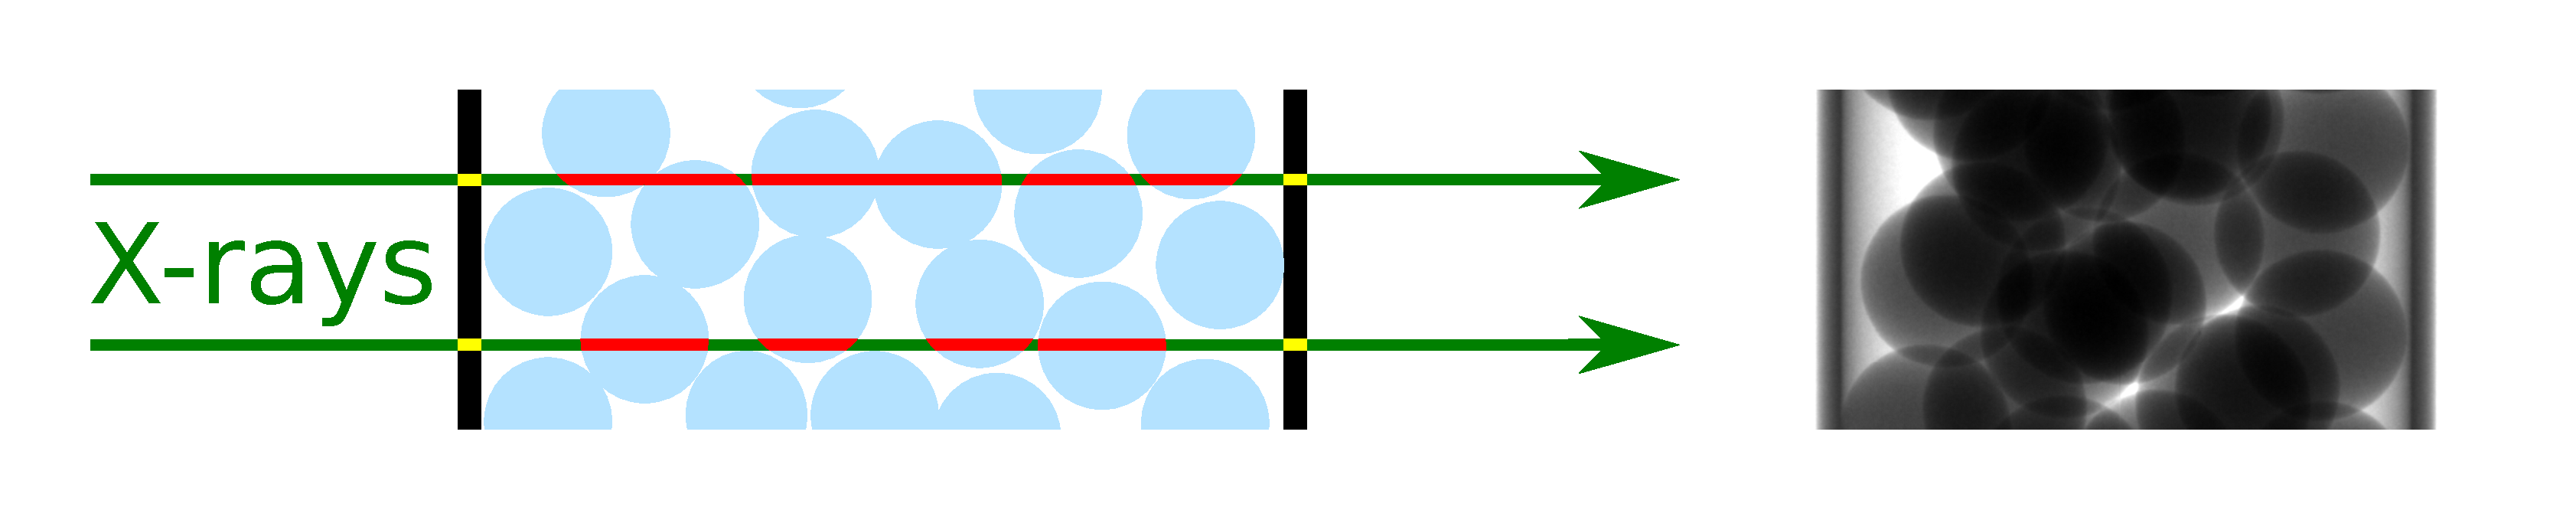
\includegraphics[width=0.8\textwidth]{Sources/beam_hardening/2beams_attenuation_marked.pdf}
\end{textblock}

\begin{textblock}{0.9}(0.05,0.7)
\visible<1->{
\centering
\Huge{
	\textcolor{white}{Correction of beam hardening \\
		in X-ray radiograms}}}
\end{textblock}

\begin{textblock}{0.9}(0.05,0.95)
	\visible<1->{
	\centering
	{
	\textcolor{white}{In collaboration with Norman Uhlmann, Fraunhofer EZRT}}}
\end{textblock}
}


%% ------------------ ATTENUATION OF X-RAYS -----------------------
\frame{
\begin{tikzpicture}[remember picture,overlay]
\fill[blue1]
(current page.north west) rectangle ([xshift=0.33\paperwidth,yshift=0.33\paperheight]current page.west|-{pic cs:end});
\end{tikzpicture}

\begin{textblock}{0.5}(0.02,0.03)
	\textcolor{white}{
		\Large Attenuation of X-rays}
\end{textblock}

\begin{textblock}{0.45}(0.5,0.1)
\centering
Beer-Lambert's law\\[0.2cm]
\visible<1>{
$\textcolor{red}{I(x)} = \textcolor{blue}{I_0} \exp(- \mu\, x)$\\
Thickness: $x = - \frac{1}{\mu} \ln\frac{I(x)}{I_0}$}
\end{textblock}

\begin{textblock}{0.45}(0.5,0.1)
\centering
Beer-Lambert's law\\[0.2cm]
\visible<2->{
$\textcolor{red}{I(x)} = \textcolor{blue}{I_0} \exp(- \textcolor{darkgreen}{\mu(E,Z,\rho)}\, x)$\\
$\mu \neq \text{const}$\\
Thickness: \colorbox{red}{$x =\, ?$}}
\end{textblock}

\begin{textblock}{0.48}(0.5,0.3)
	\visible<2->{
	\centering
	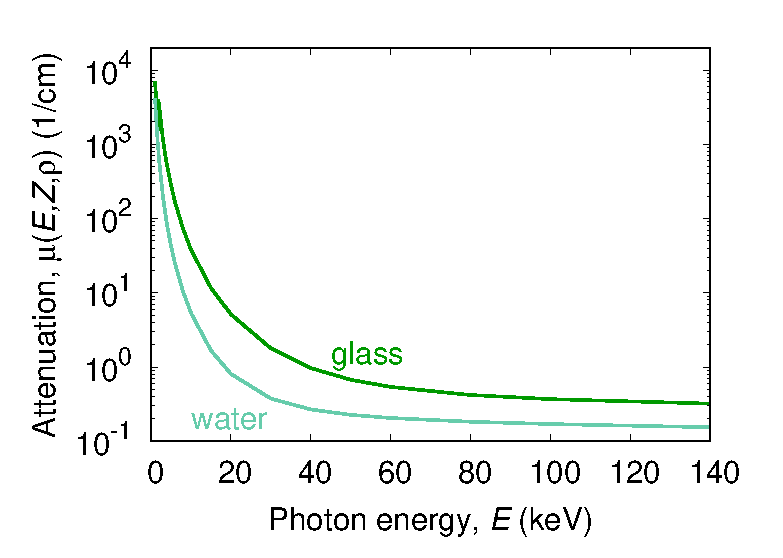
\includegraphics[width=\textwidth]
	{Sources/beam_hardening/Attenuation_vs_energy.eps}}
\end{textblock}
\begin{textblock}{0.48}(0.5,0.9)
	\centering
	\visible<2->{\scriptsize{
		\url{https://www.nist.gov/pml/x-ray-mass-attenuation-coefficients}}}
\end{textblock}

\begin{textblock}{0.45}(0.03,0.14)
	\centering
	\only<1> {%% image of beam through material
	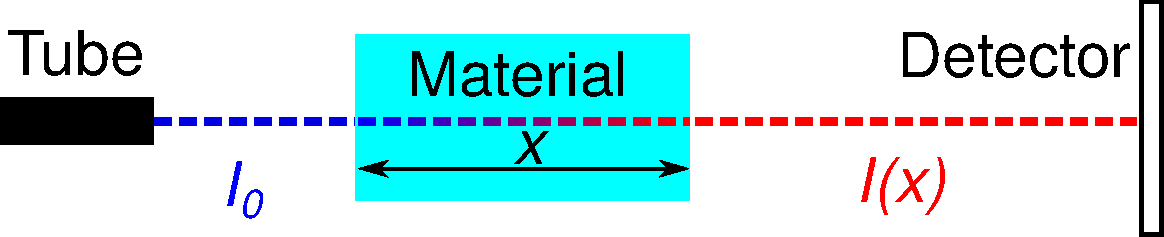
\includegraphics[width=\textwidth]
	{Sources/beam_hardening/beam_through_material.pdf}}
	\only<2>{
	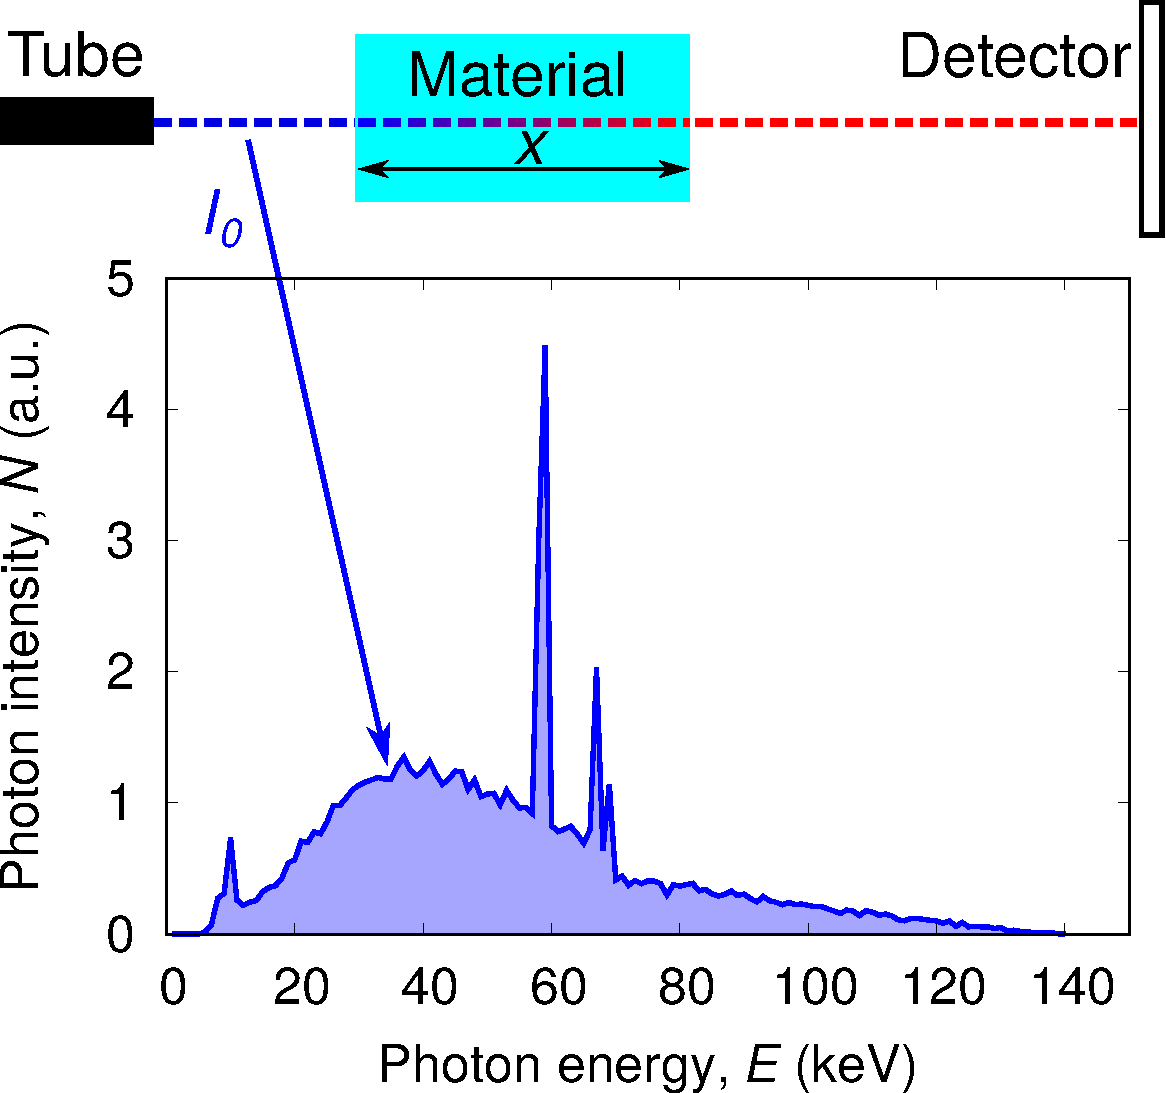
\includegraphics[width=\textwidth]
	{Sources/beam_hardening/x-ray_spectrum_N0.pdf}}
	\only<3>{
	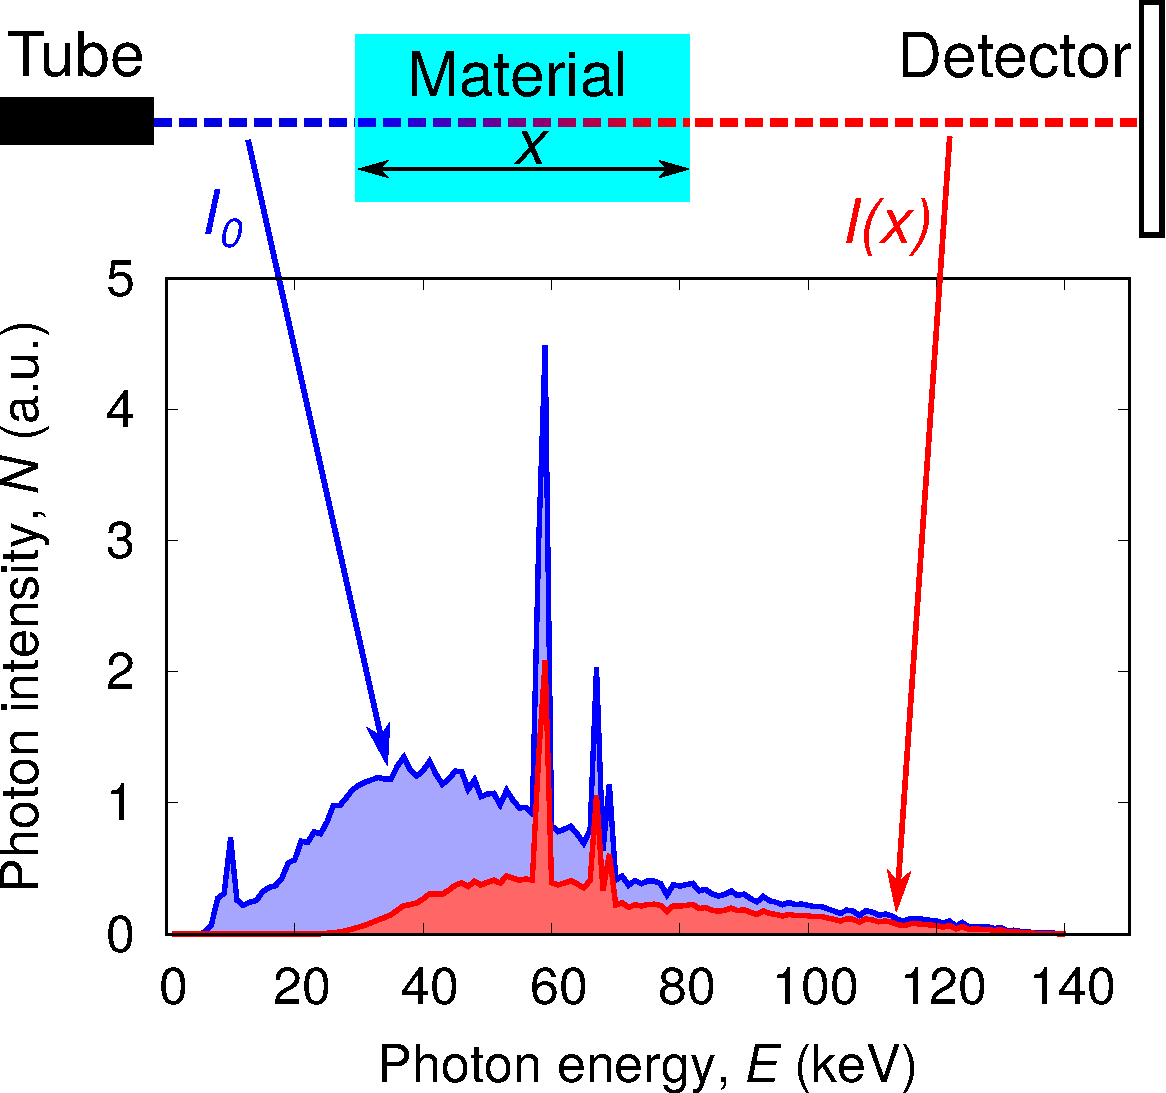
\includegraphics[width=\textwidth]
	{Sources/beam_hardening/x-ray_spectra_beam_hardening.pdf}}
\end{textblock}
\begin{textblock}{0.45}(0.035,0.36)
	\centering
	\only<3>{
	\colorbox{red}{Beam hardening}}
\end{textblock}

\note{Attenuation of X-rays}


}




%%%-------------- ENERGY AVERAGED ATTENUATION ----------------
\frame{
\begin{tikzpicture}[remember picture,overlay]
\fill[blue1]
(current page.north west) rectangle ([xshift=0.45\textwidth,yshift=0.33\textheight]current page.west|-{pic cs:end});
\end{tikzpicture}

\begin{textblock}{0.5}(0.02,0.03)
	\textcolor{white}{
		\Large The effective attenuation, $\mu_\text{eff}$}
\end{textblock}


\begin{textblock}{0.45}(0.03,0.1)
	\centering
	\only<1>{
	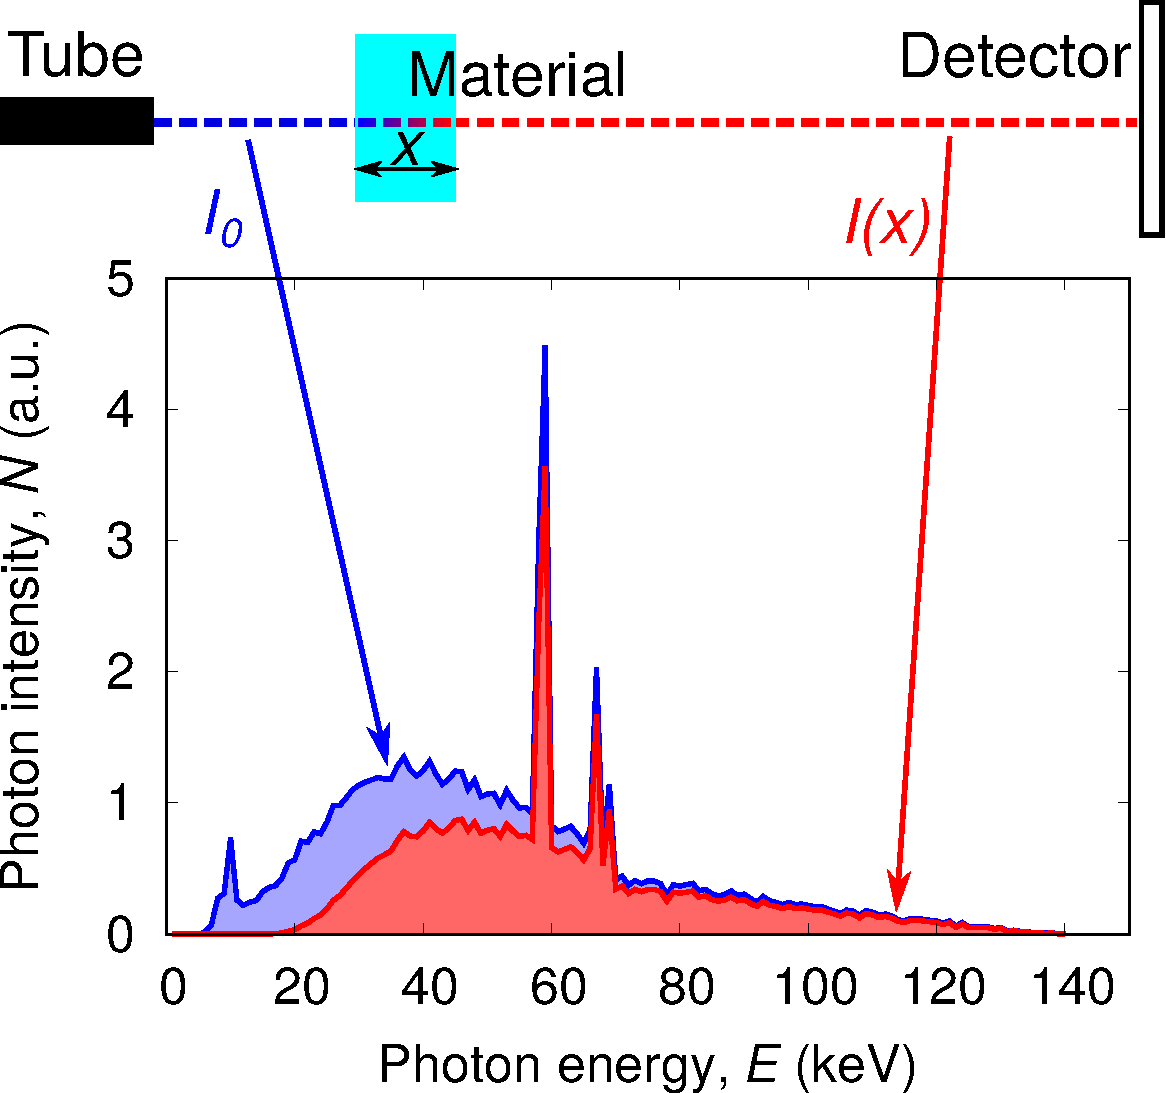
\includegraphics[width=\textwidth]
	{Sources/beam_hardening/x-ray_spectra_beam_hardening_step1.pdf}}
	\only<2>{
	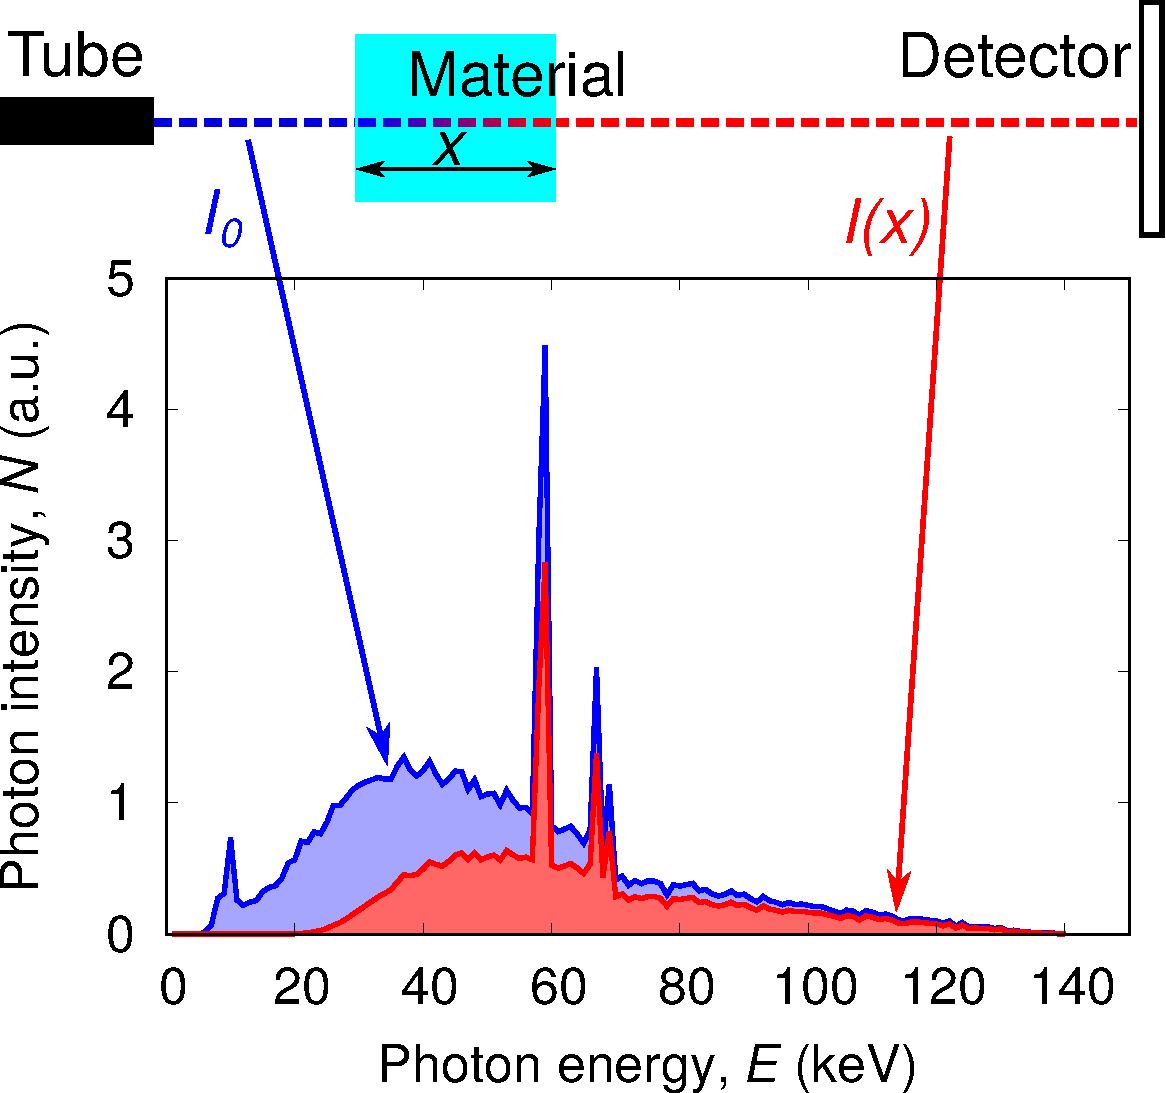
\includegraphics[width=\textwidth]
	{Sources/beam_hardening/x-ray_spectra_beam_hardening_step2.pdf}}
	\only<3,4>{
	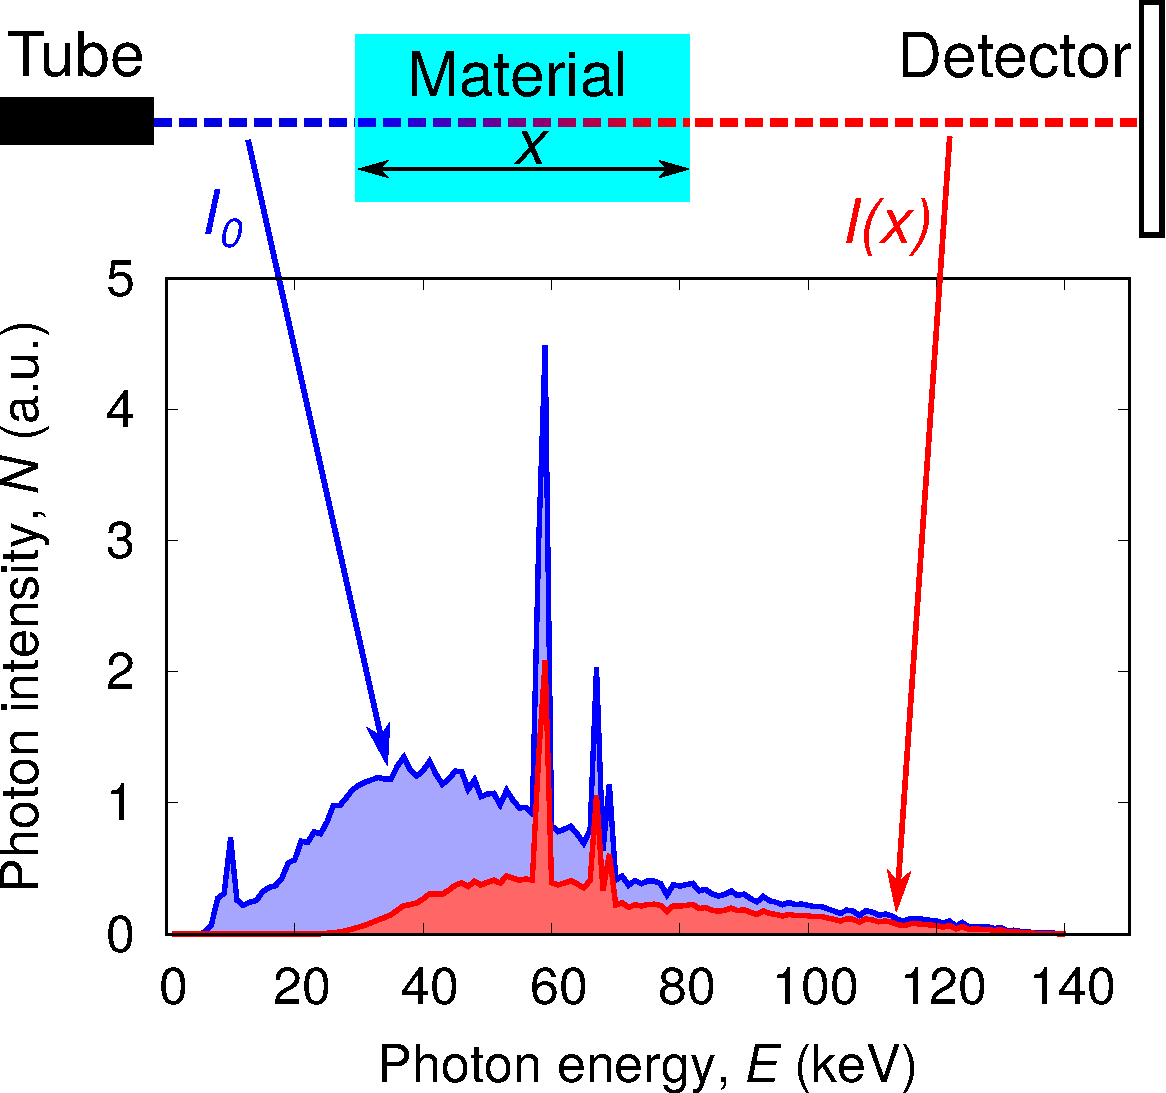
\includegraphics[width=\textwidth]
	{Sources/beam_hardening/x-ray_spectra_beam_hardening.pdf}}
\end{textblock}

\begin{textblock}{0.17}(0.5,0.02)
	\only<1>{
	\fbox{
	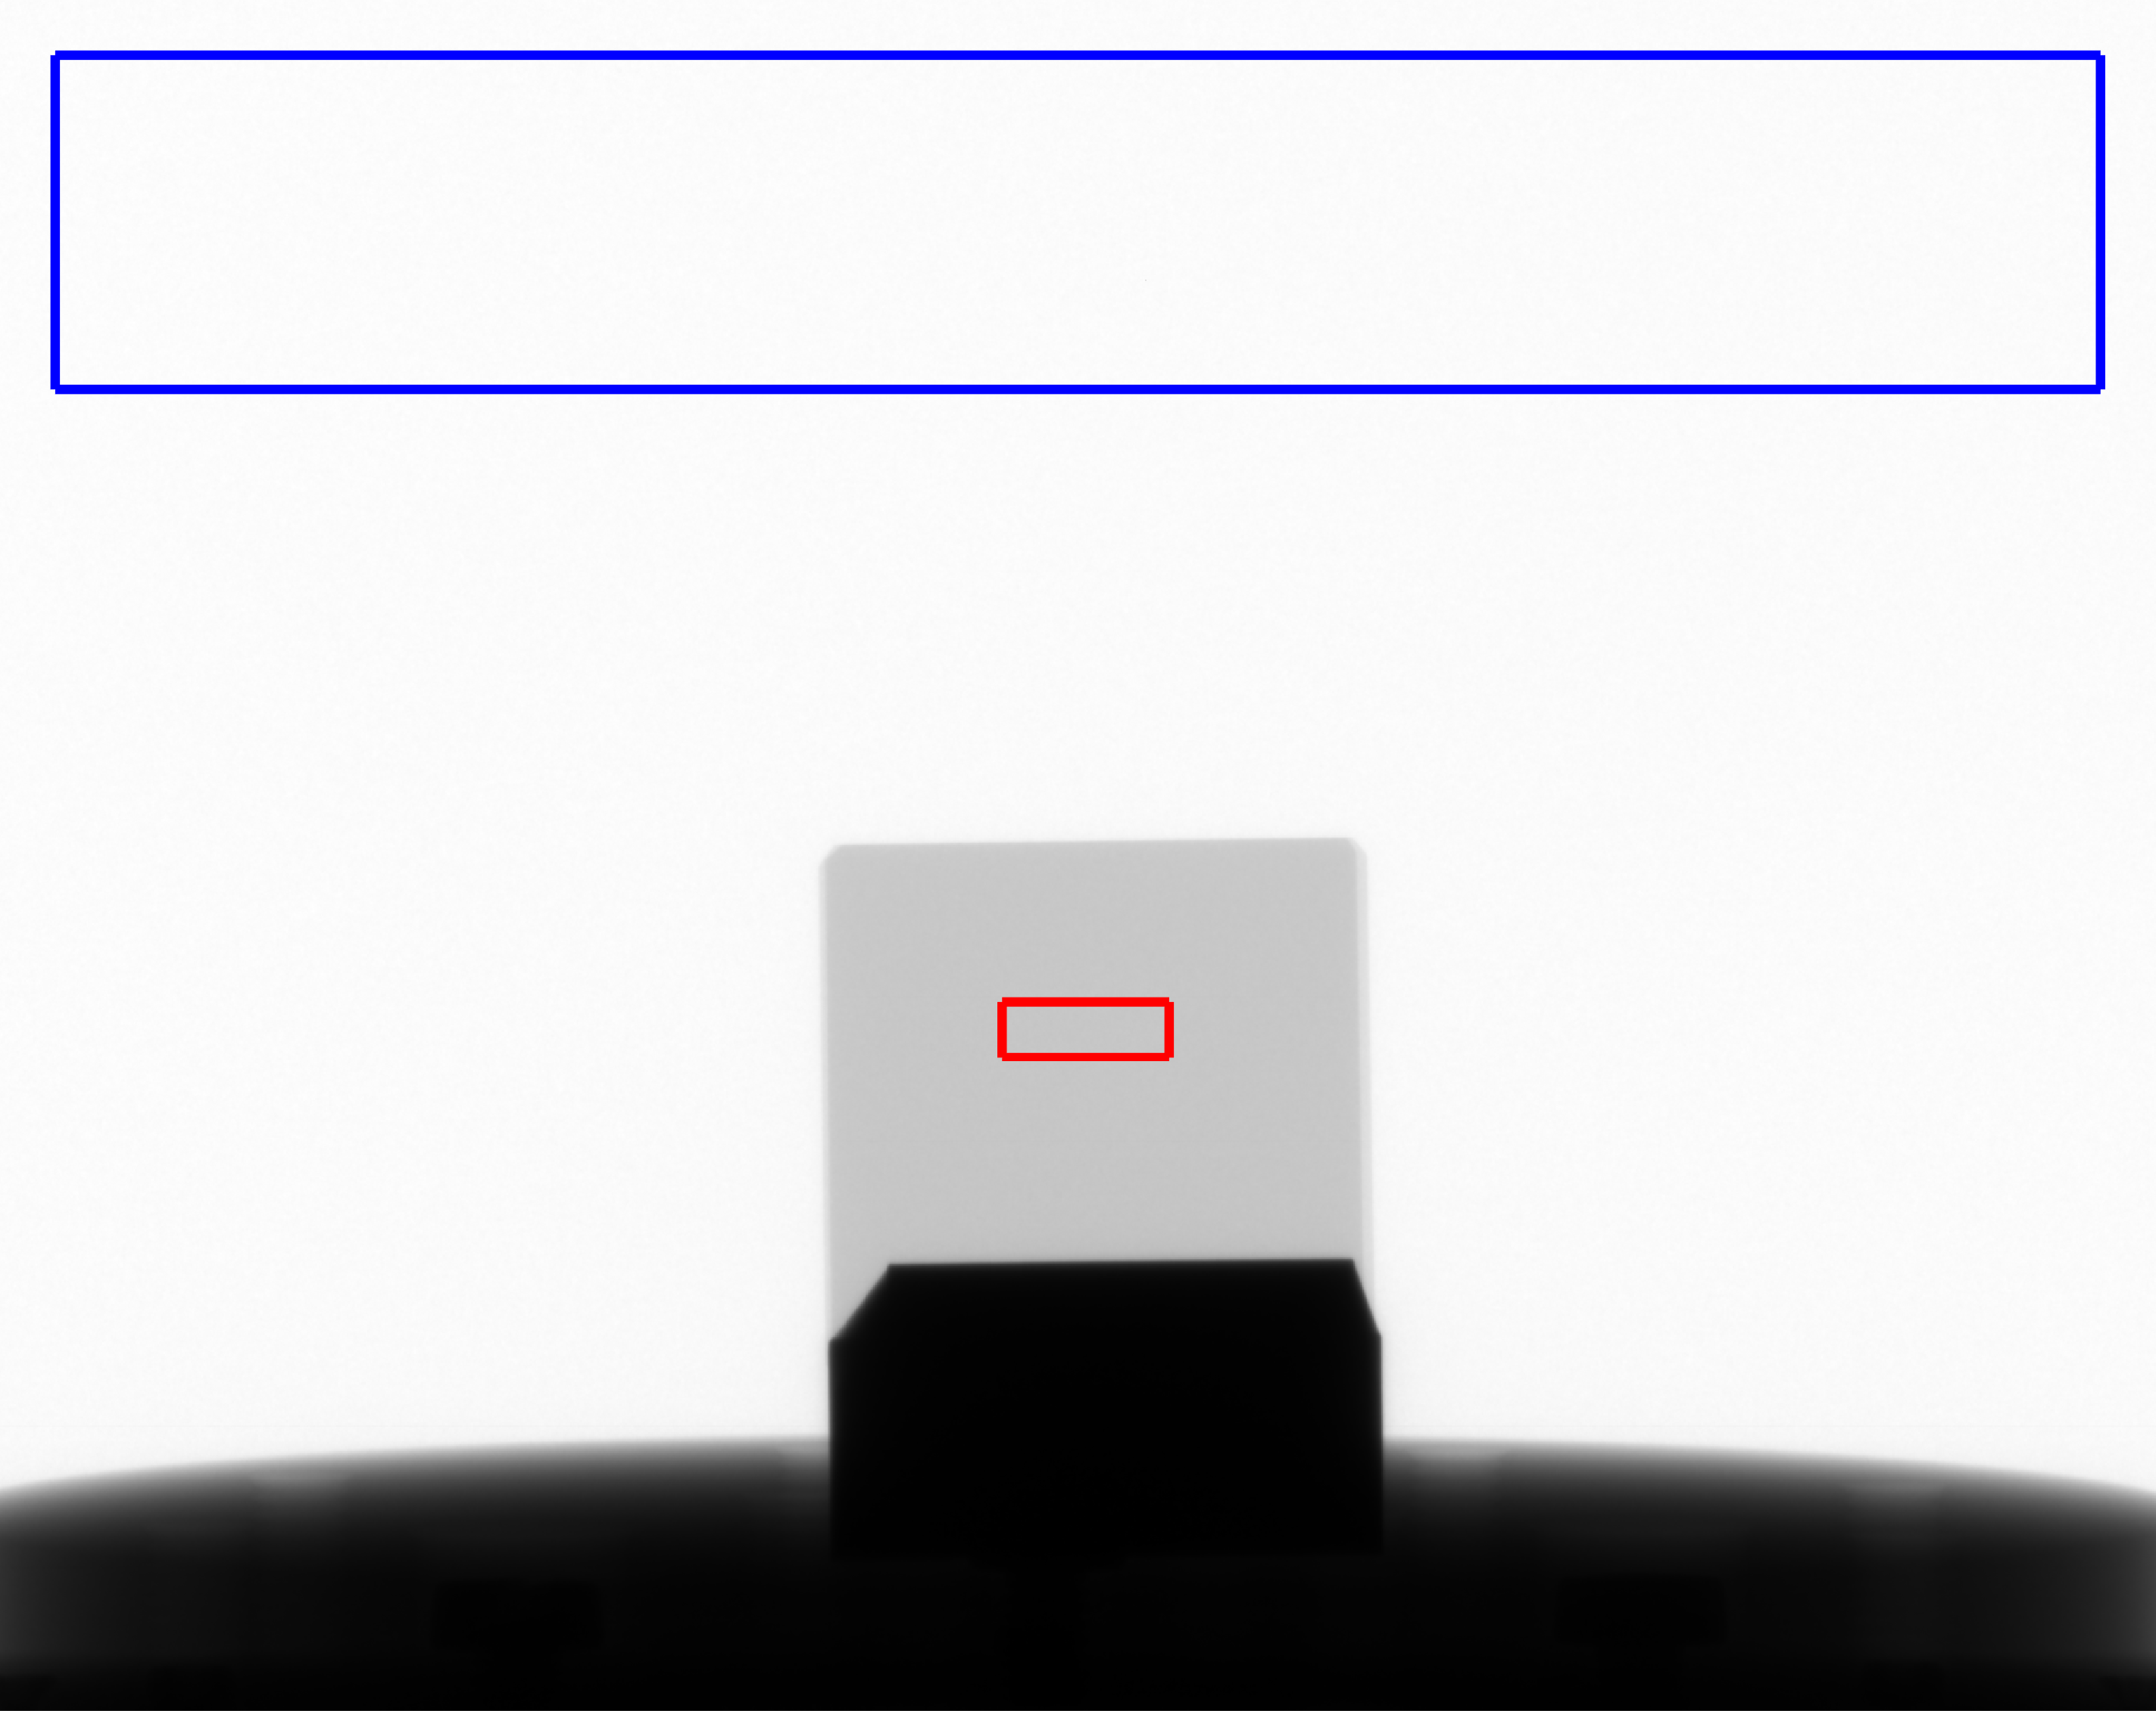
\includegraphics[width=\textwidth]
	{Sources/beam_hardening/02_plates.png}}}
	\only<2>{
	\fbox{
	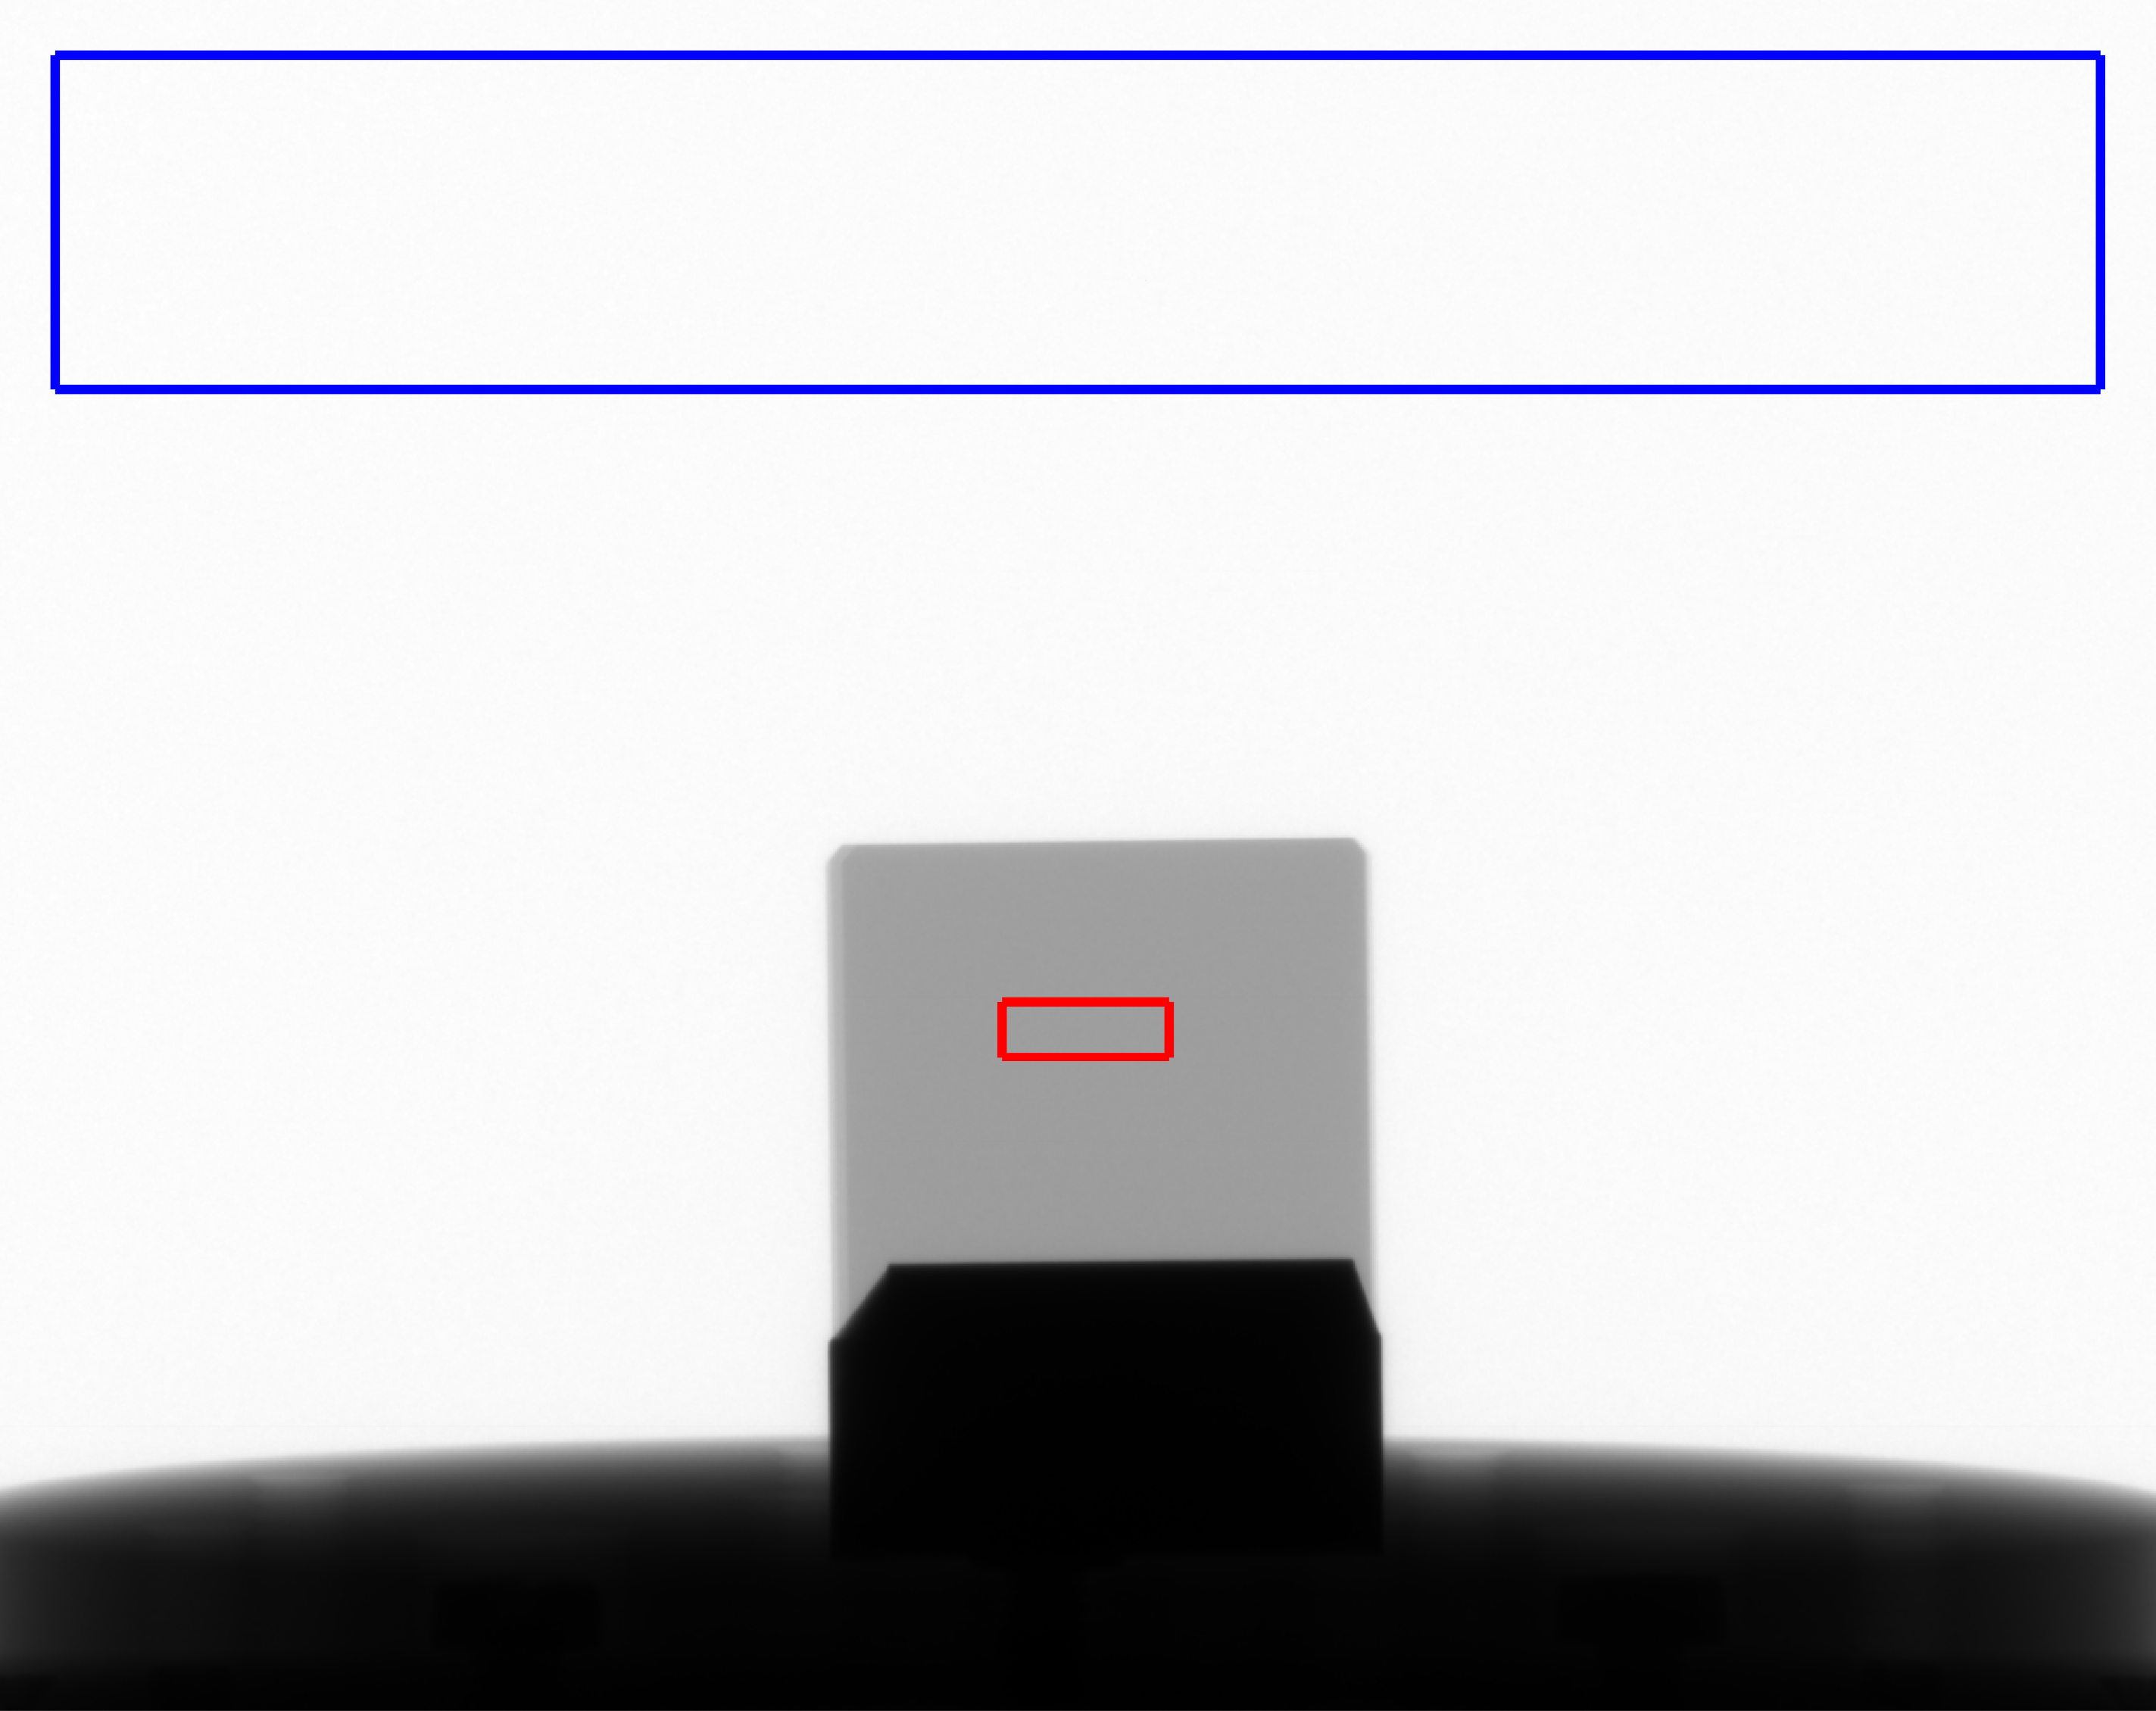
\includegraphics[width=\textwidth]
	{Sources/beam_hardening/04_plates.png}}}
	\only<3,4>{
	\fbox{
	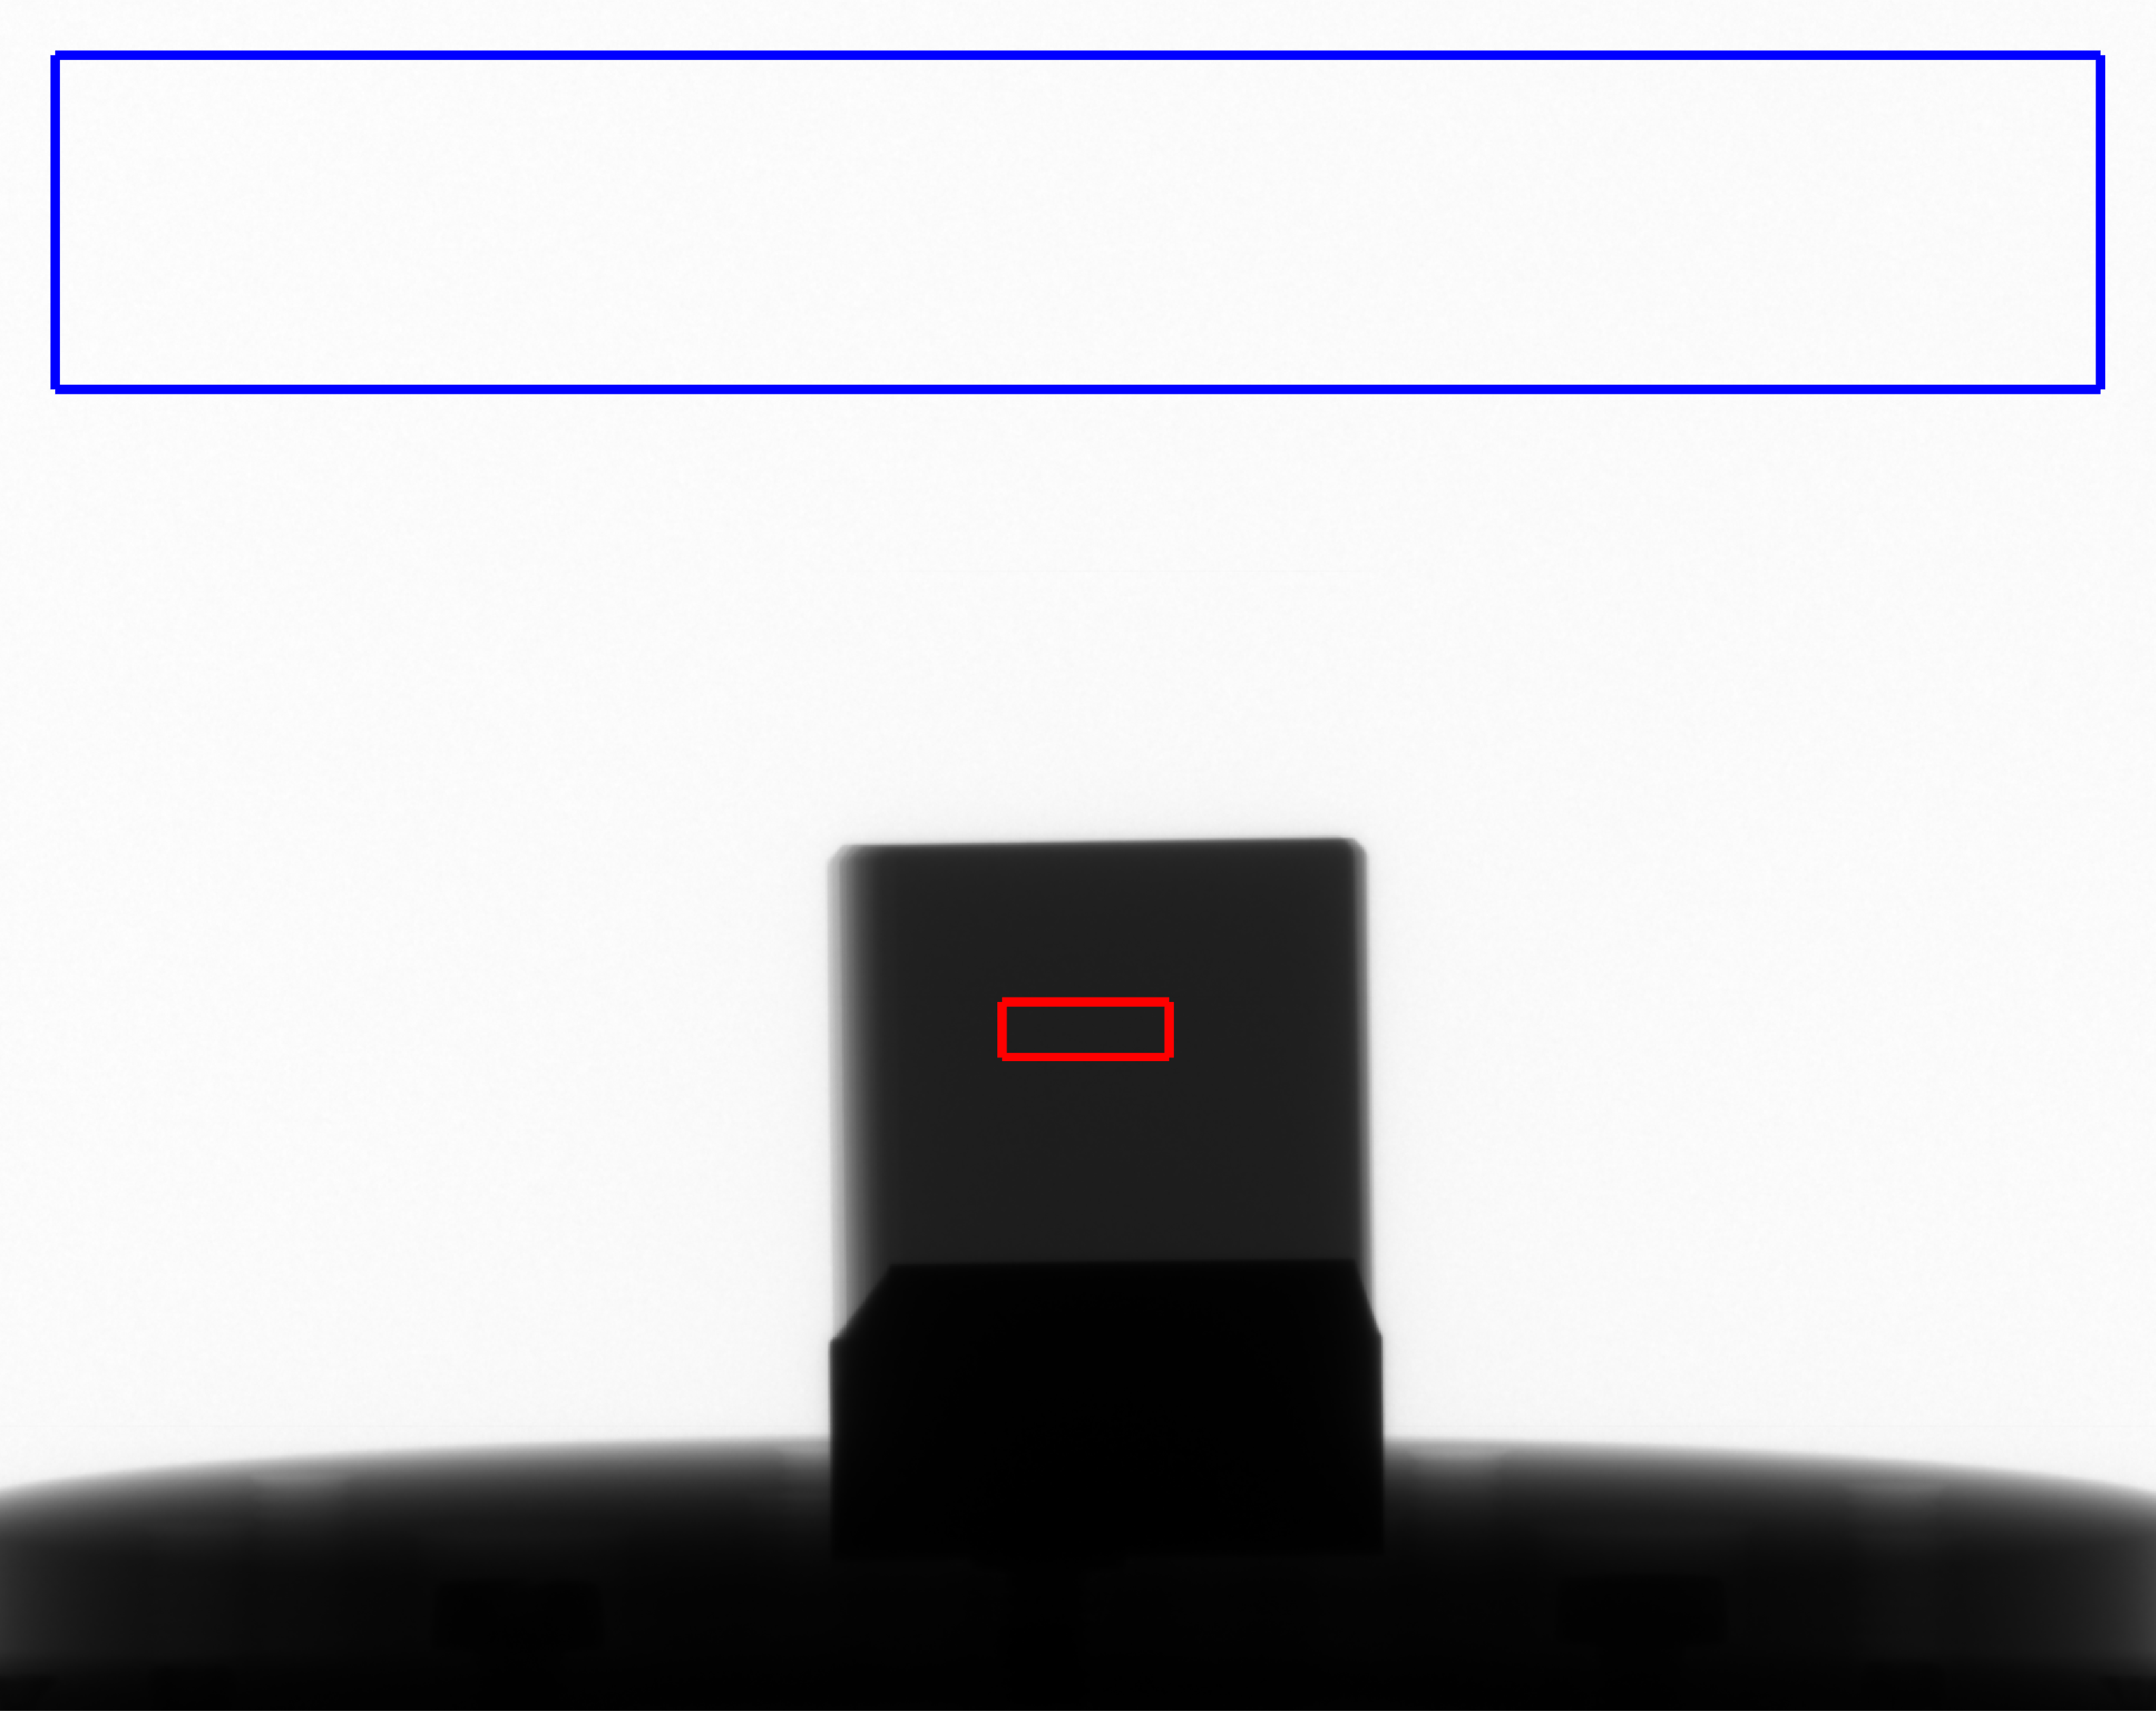
\includegraphics[width=\textwidth]
	{Sources/beam_hardening/20_plates.png}}}
\end{textblock}

\begin{textblock}{0.28}(0.7,0.05)
	\visible<1->{
		\textcolor{darkgreen}{\textit{effective}} attenuation: \\
		$\textcolor{red}{I(x)} = \textcolor{blue}{I_0} \exp(- \textcolor{darkgreen}{\mu_\text{eff}(x)}\, x)$}
	\visible<4->{
		\[ \textcolor{darkgreen}{\mu_\text{eff} (x)} = - 
		\frac{1}{x} 
		\frac{\textcolor{red}{I(x)}}{\textcolor{blue}{I_0}}\]}
\end{textblock}


\begin{textblock}{0.48}(0.5,0.3)
	\visible<4->{
	\includegraphics[width=\textwidth]
	{Sources/beam_hardening/attenuation_boro_glass_140kV.pdf}}
\end{textblock}

\begin{textblock}{0.15}(0.8,0.4)
	\centering
	\visible<4->{
	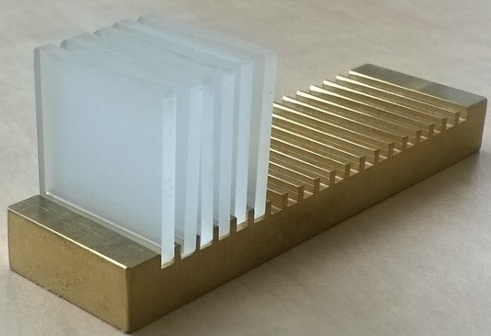
\includegraphics[width=\textwidth]
	{Sources/beam_hardening/plates_on_slide.png}}
\end{textblock}


}





%%%%%%%%%%%%%%%%%%%% Modeling mu_eff %%%%%%%%%%%%%%%%%%%%%%%%%%%%
\frame{
\begin{tikzpicture}[remember picture,overlay]
\fill[blue1]
(current page.north west) rectangle ([xshift=0.23\textwidth,yshift=0.33\textheight]current page.west|-{pic cs:end});
\end{tikzpicture}

\begin{textblock}{0.22}(0.0,0.03)
	\centering
	\textcolor{white}{
		\Large Modeling of $\mu_\text{eff}$}
\end{textblock}



\begin{textblock}{1.}(0.0,0.03)
	\centering
	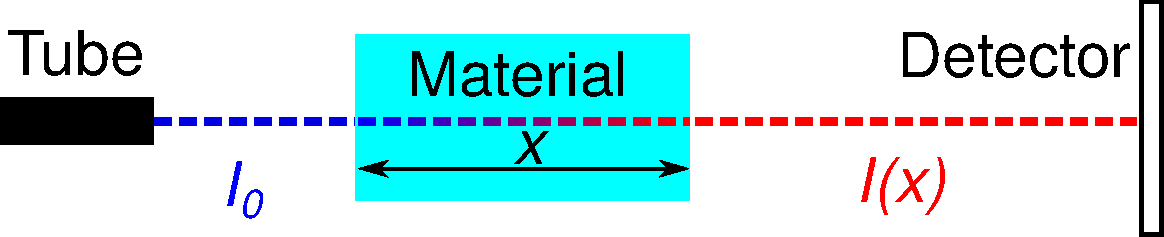
\includegraphics[width=0.4\textwidth]
	{Sources/beam_hardening/beam_through_material.pdf}
\end{textblock}

%% Photon spectrum
\begin{textblock}{0.32}(0.03,0.18)
	\centering
	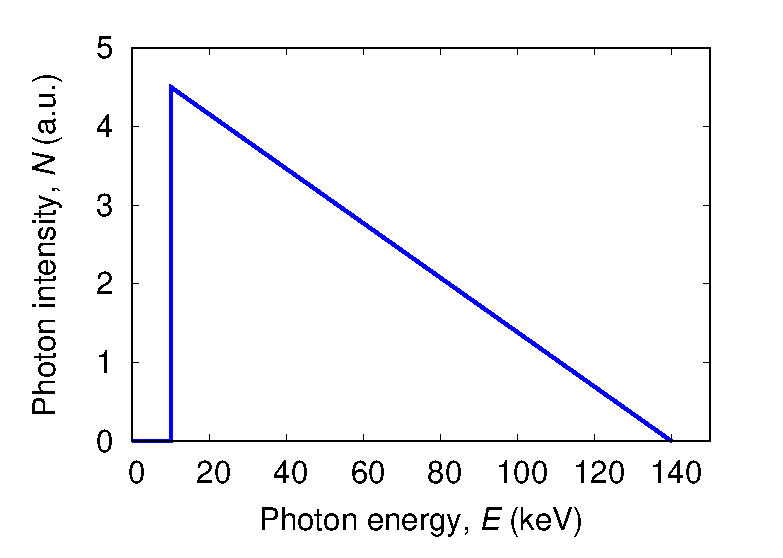
\includegraphics[width=\textwidth]
	{Sources/beam_hardening/linear_spectrum.eps}
\end{textblock}

\begin{textblock}{0.32}(0.03,0.17)
	\centering
	\hspace{0.5cm}
	\pgfsetfillopacity{1}\colorbox{blue1}{\pgfsetfillopacity{1}\textcolor{white}{
			$N (E) = -a E + b$}}
\end{textblock}

%% attenuation data
\begin{textblock}{0.32}(0.345,0.18)
	\centering
	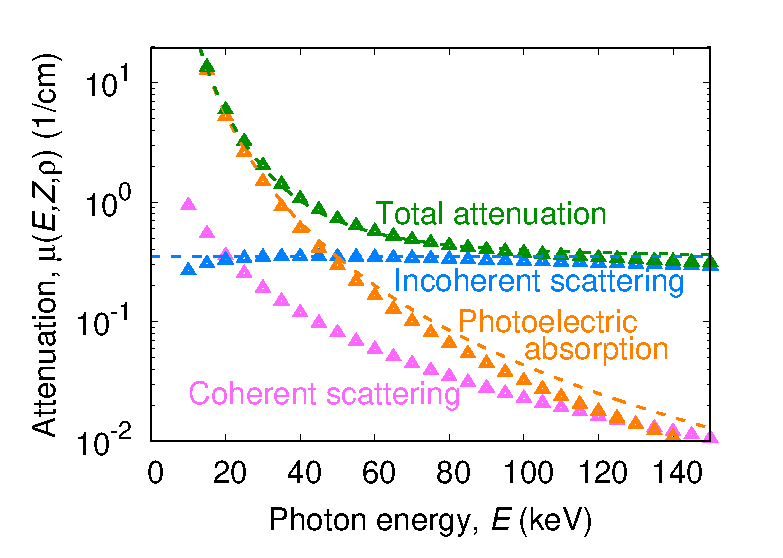
\includegraphics[width=\textwidth]
	{Sources/beam_hardening/XCOM_attenuation.eps}
\end{textblock}

\begin{textblock}{0.32}(0.345,0.17)
	\centering
	\hspace{0.5cm}
	\pgfsetfillopacity{1}\colorbox{darkgreen}{\pgfsetfillopacity{1}\textcolor{white}{
			$\mu (E) = \mu_\text{C} + c E^{-3}~\,^{(*)}$}}
\end{textblock}

%% detector curve
\begin{textblock}{0.32}(0.67,0.18)
	\centering
	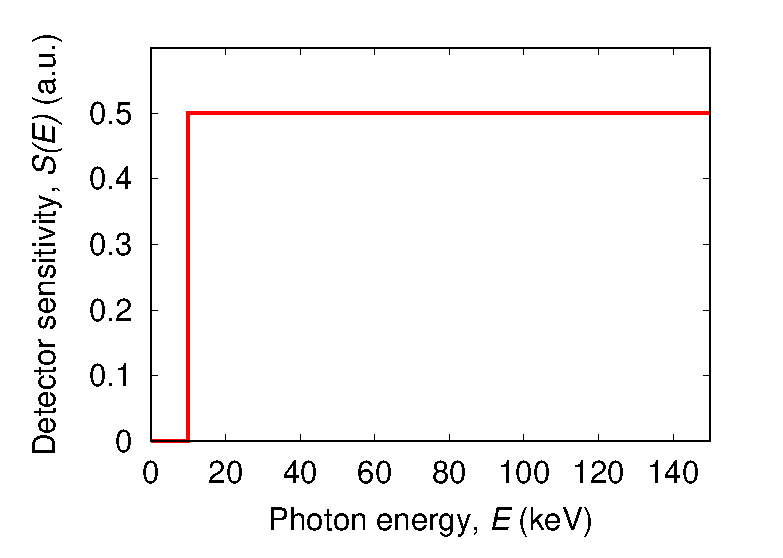
\includegraphics[width=\textwidth]
	{Sources/beam_hardening/detector_const.eps}
\end{textblock}

\begin{textblock}{0.32}(0.67,0.17)
	\centering
	\hspace{0.5cm}
	\pgfsetfillopacity{1}\colorbox{red}{\pgfsetfillopacity{1}\textcolor{white}{
		$S(E) = S~\Theta(E - E_\text{min})$}}
\end{textblock}


\begin{textblock}{0.5}(0.05,0.7)
	\visible<1->{
		$I(x) \propto \int \textcolor{blue}{N(E)} \exp\{-
		\textcolor{darkgreen}{\mu(E,Z,\rho)} x\} 
		\textcolor{red}{S(E)}~\mathrm{d}E $}
\end{textblock}

\begin{textblock}{0.32}(0.55,0.58)
	\visible<2->{
		\centering
		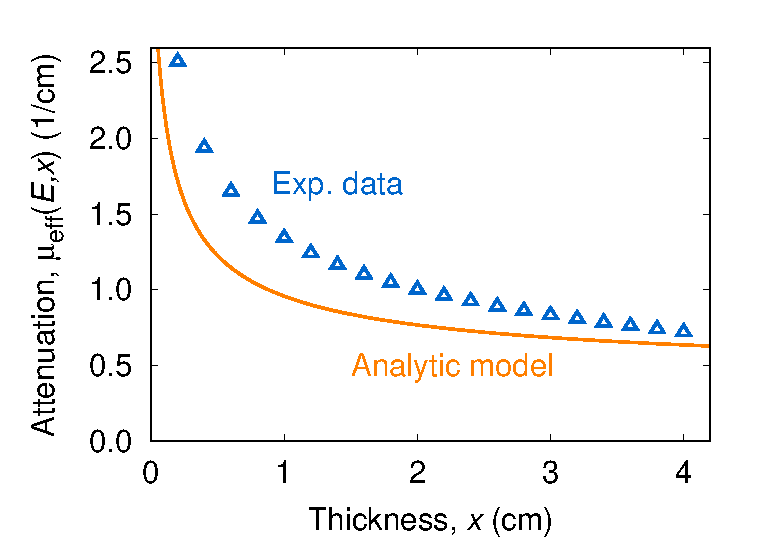
\includegraphics[width=\textwidth]
		{Sources/beam_hardening/attenuation_borosilicate_glass_voltages_first_principle_fit.eps}
	}
\end{textblock}

\begin{textblock}{0.9}(0.02,0.93)
	{\scriptsize
		$(*)$ XCOM supplied by NIST}
\end{textblock}

\begin{textblock}{1.}(0,0)
	\visible<3->{
		
\includegraphics[width=\textwidth]
		{Sources/beam_hardening/cross.pdf}}
\end{textblock}
}



%%%%%%%%%%%%%%%%%% Numerical approach %%%%%%%%%%%%%%%%%%%%%%%%%%%%
\frame{
\begin{tikzpicture}[remember picture,overlay]
\fill[blue1]
(current page.north west) rectangle ([xshift=0.23\textwidth,yshift=0.27\textheight]current page.west|-{pic cs:end});
\end{tikzpicture}

\begin{textblock}{0.22}(0.0,0.03)
	\centering
	\textcolor{white}{
	\Large Numerical approx.\ of 
	$\mu_\text{eff}$}
\end{textblock}



\begin{textblock}{1.}(0.0,0.03)
	\centering
	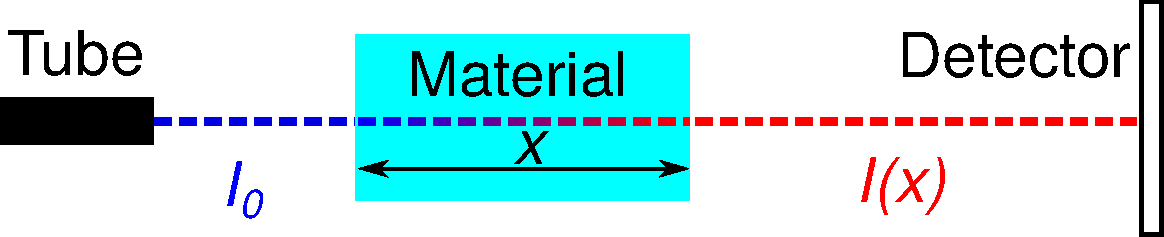
\includegraphics[width=0.4\textwidth]
	{Sources/beam_hardening/beam_through_material.pdf}
\end{textblock}

%% Photon spectrum
\begin{textblock}{0.32}(0.03,0.18)
	\centering
	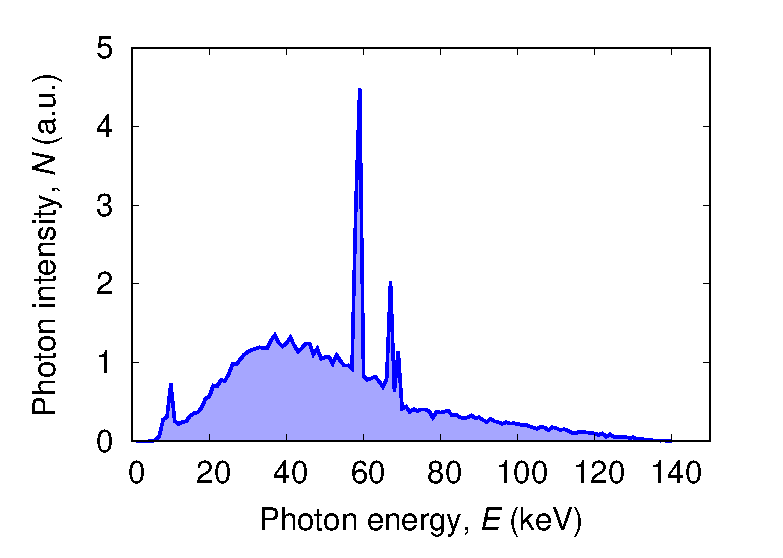
\includegraphics[width=\textwidth]
	{Sources/beam_hardening/N0_initial_spectrum_filled_curves.eps}
\end{textblock}

\begin{textblock}{0.32}(0.03,0.18)
	\centering
	\vspace{0.1cm}	
	\pgfsetfillopacity{0.85}\colorbox{blue1}{\pgfsetfillopacity{1}\textcolor{white}{
			Comet X-ray tube$^{(1)}$}}
\end{textblock}

%% attenuation data
\begin{textblock}{0.32}(0.345,0.18)
	\centering
	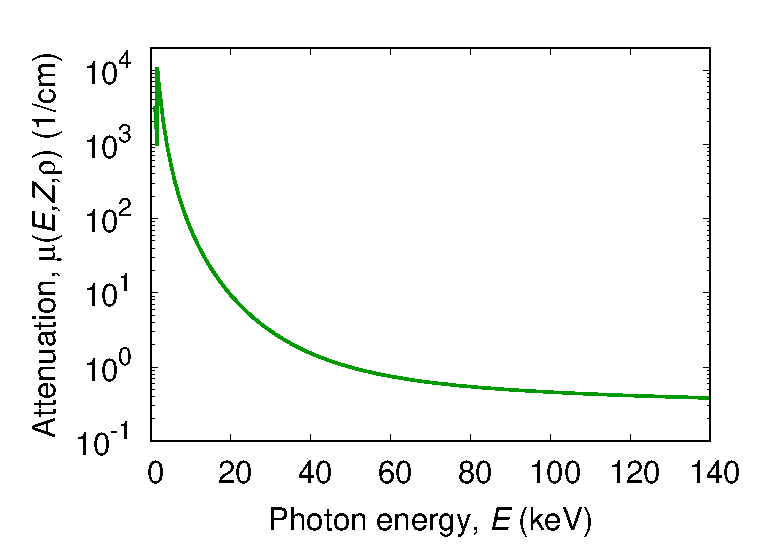
\includegraphics[width=\textwidth]
	{Sources/beam_hardening/Attenuation_vs_energy_Al.eps}
\end{textblock}

\begin{textblock}{0.32}(0.345,0.18)
	\centering
	\vspace{0.1cm}
	\pgfsetfillopacity{0.85}\colorbox{blue1}{\pgfsetfillopacity{1}\textcolor{white}{
			Aluminum$^{(2)}$}}
\end{textblock}

%% detector curve
\begin{textblock}{0.32}(0.67,0.18)
	\centering
		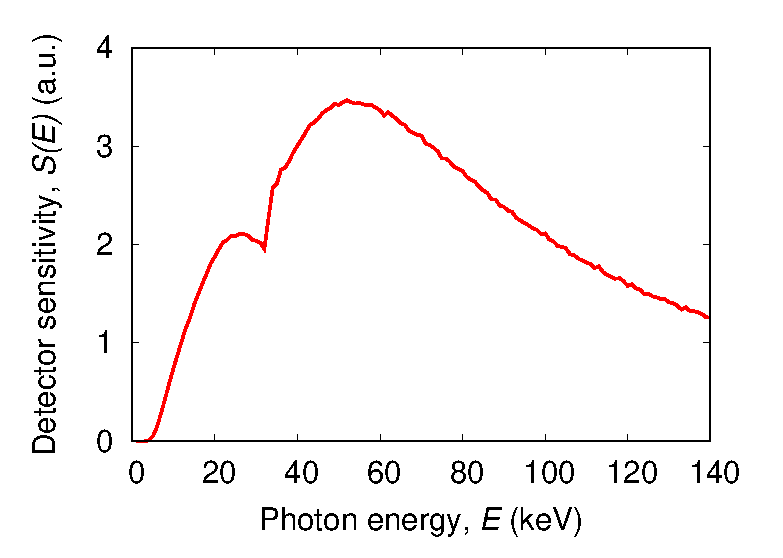
\includegraphics[width=\textwidth]
		{Sources/beam_hardening/Detector_response_0.eps}
\end{textblock}

\begin{textblock}{0.32}(0.67,0.18)
	\centering
	\vspace{0.1cm}
	\pgfsetfillopacity{0.85}\colorbox{blue1}{\pgfsetfillopacity{1}\textcolor{white}{
			XEye detector$^{(1)}$}}
\end{textblock}


\begin{textblock}{0.5}(0.05,0.7)
	\visible<1->{
		$I(x) \propto \int \textcolor{blue}{N(E)} \exp\{-
		\textcolor{darkgreen}{\mu(E,Z,\rho)} x\} 
		\textcolor{red}{S(E)}~\mathrm{d}E $}
%	\visible<2->{
%		\[ \textcolor{darkgreen}{\mu_\text{eff} (x)} = - 
%		\frac{1}{x} 
%		\frac{\textcolor{red}{I(x)}}{\textcolor{blue}{I_0}}\]}
\end{textblock}

\begin{textblock}{0.32}(0.55,0.58)
	\visible<2->{
	\centering
	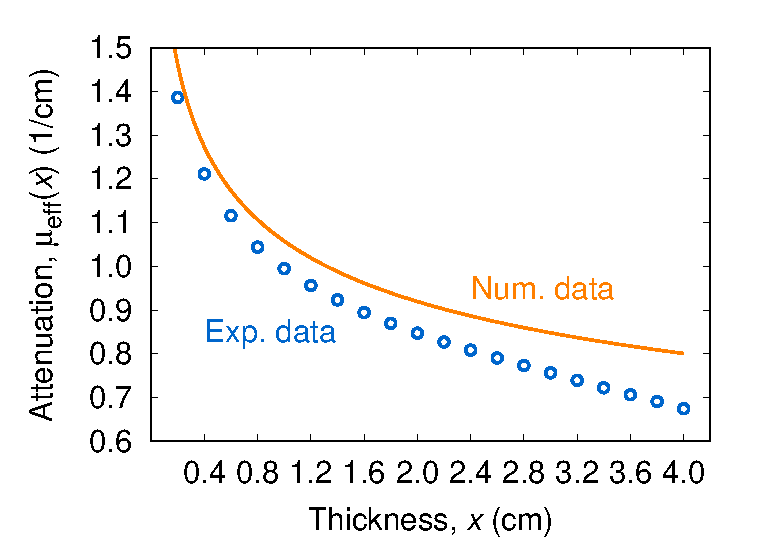
\includegraphics[width=\textwidth]
	{Sources/beam_hardening/mu_eff_140kV_exp_vs_numeric_data_norman.eps}
	}
\end{textblock}

\begin{textblock}{0.9}(0.02,0.9)
{\scriptsize
$(1)$ Supplied by Norman Uhlmann, Fraunhofer EZRT\\
$(2)$ XCOM supplied by NIST}
\end{textblock}

\begin{textblock}{1.}(0,0)
	\visible<3->{
	
\includegraphics[width=\textwidth]
{Sources/beam_hardening/cross.pdf}}
\end{textblock}
}




%% ------------- HEURISTIC MODEL-FUNCTION ------------
\frame{
\begin{tikzpicture}[remember picture,overlay]
\fill[blue1]
(current page.north west) rectangle ([xshift=0.5\textwidth,yshift=0.34\textheight]current page.west|-{pic cs:end});
\end{tikzpicture}

\begin{textblock}{0.5}(0.02,0.03)
	\textcolor{white}{
		\Large Heuristic model functions for $\mu_\text{eff}$}
\end{textblock}

\begin{textblock}{0.4}(0.03,0.08)
	\only<1>{
	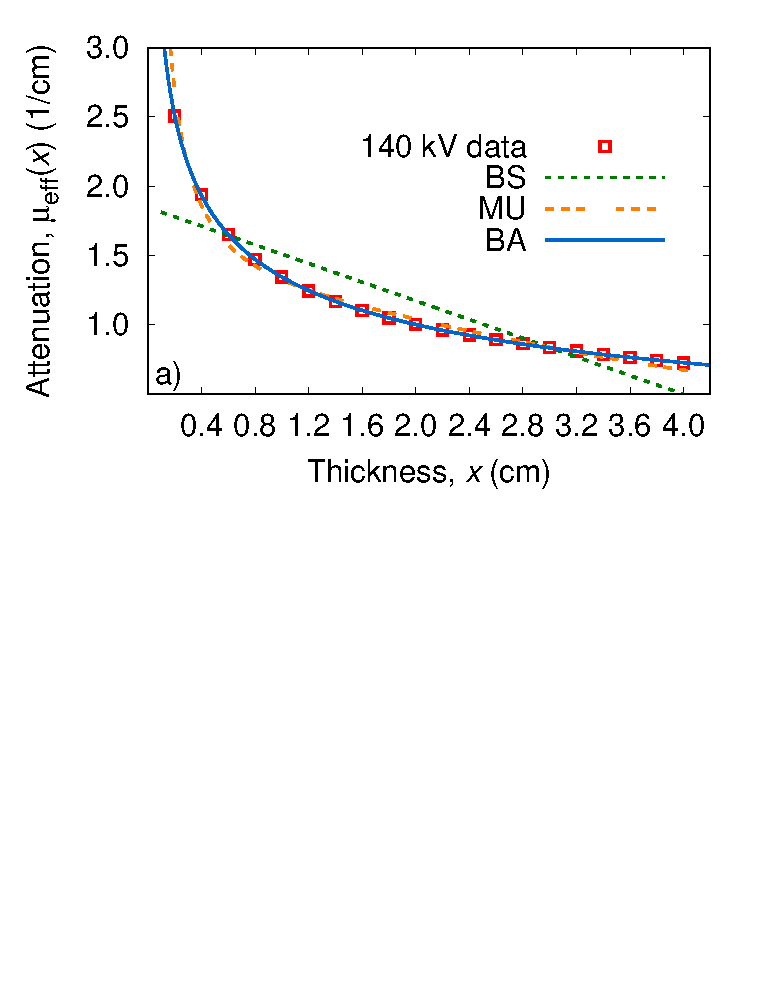
\includegraphics[width=\textwidth]
	{Sources/beam_hardening/borosilicate_glass_140kV_model_comparison_upper_plot.eps}}
	\visible<2->{
	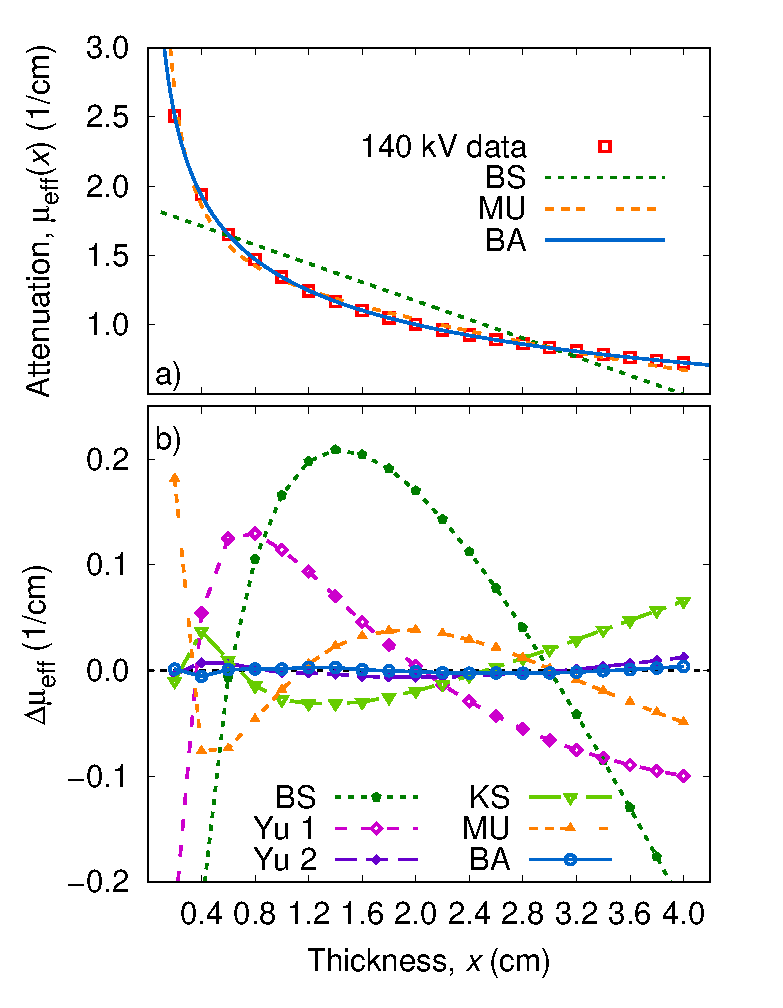
\includegraphics[width=\textwidth]
	{Sources/beam_hardening/borosilicate_glass_140kV_model_comparison_multiplot.eps}}
\end{textblock}


\begin{textblock}{0.5}(0.4, 0.12)
\begin{tabular}{ll}
{\small
	\textcolor{BS}{$\mu_\text{eff} (x)= \mu_0 - \lambda x$}} &
	{\small Bjärngard \& Shackford} \\
		& {\small (1994)}\\[0.7cm]
	
{\small	
\textcolor{Yu1}{$\mu_\text{eff}(x) = \frac{\mu_0}{1+\lambda x}$}} &
\multirow{2}{\linewidth}{\small Yu \textit{et al.} (1997)}\\

{\small
\textcolor{Yu2}{$\mu_\text{eff}(x) = \frac{\mu_0}{(1+\lambda x)^\beta}$}} \\[0.7cm]

{\small
\textcolor{KS}{
	$\mu_\text{eff}(x) = \mu(E_\text{max}) +
	\frac{2 \mu_1}{x \sqrt{-\lambda_1^2 + 4 \lambda_2}} \times$}} & Kleinschmidt (1999)
\\
\multicolumn{2}{l}{\small
\textcolor{KS}{
	$\quad\left[
	\arctan\left(
	\frac{\lambda_1 + 2 \lambda_2 x}{\sqrt{-\lambda_1^2 + 4 \lambda_2}}
	\right)
	-\arctan\left(
	\frac{\lambda_1}{\sqrt{-\lambda_1^2 + 4 \lambda_2}}
	\right)
	\right]
	$ }} \\[0.7cm]

{\small
\textcolor{MU}{$\mu_\text{eff}(x) = -\frac{1}{x} \ln \left[A+B \exp(-x/C)\right]$}} & 
{\small
	Mudde \textit{et al.} (2008) }\\[0.7cm]

{\small
\textcolor{BA}{$\boldsymbol{\mu_\text{eff}(x) = a + \frac{b}{x^\alpha}}$}} &
{\small \textbf{Baur \textit{et al.} (2019)}}\\
& {\small (this work)}
\end{tabular}

\end{textblock}
f}

%% ------------- RESULTS -----------------------------
\frame{
\begin{tikzpicture}[remember picture,overlay]
\fill[blue1]
(current page.north west) rectangle ([xshift=0.22\textwidth,yshift=-10.cm]current page.west|-{pic cs:end});
\end{tikzpicture}

\begin{textblock}{0.2}(0.01,0.15)
	\textcolor{white}{\Large
	{Universality of }{\large$\boldsymbol{\mu_\text{eff}(x) = a + \frac{b}{x^\alpha}}$}}
\end{textblock}

\begin{textblock}{0.2}(0.005,0.35)
	\centering
	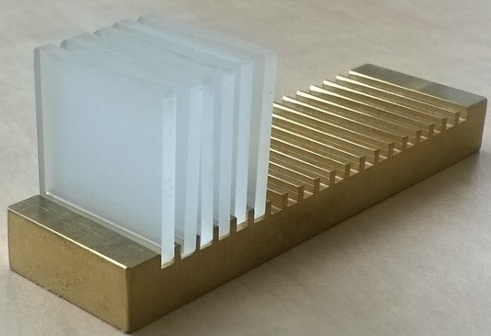
\includegraphics[width=0.8\textwidth]
	{Sources/beam_hardening/plates_on_slide.png}
\end{textblock}

\begin{textblock}{0.2}(0.005,0.65)
	\centering
	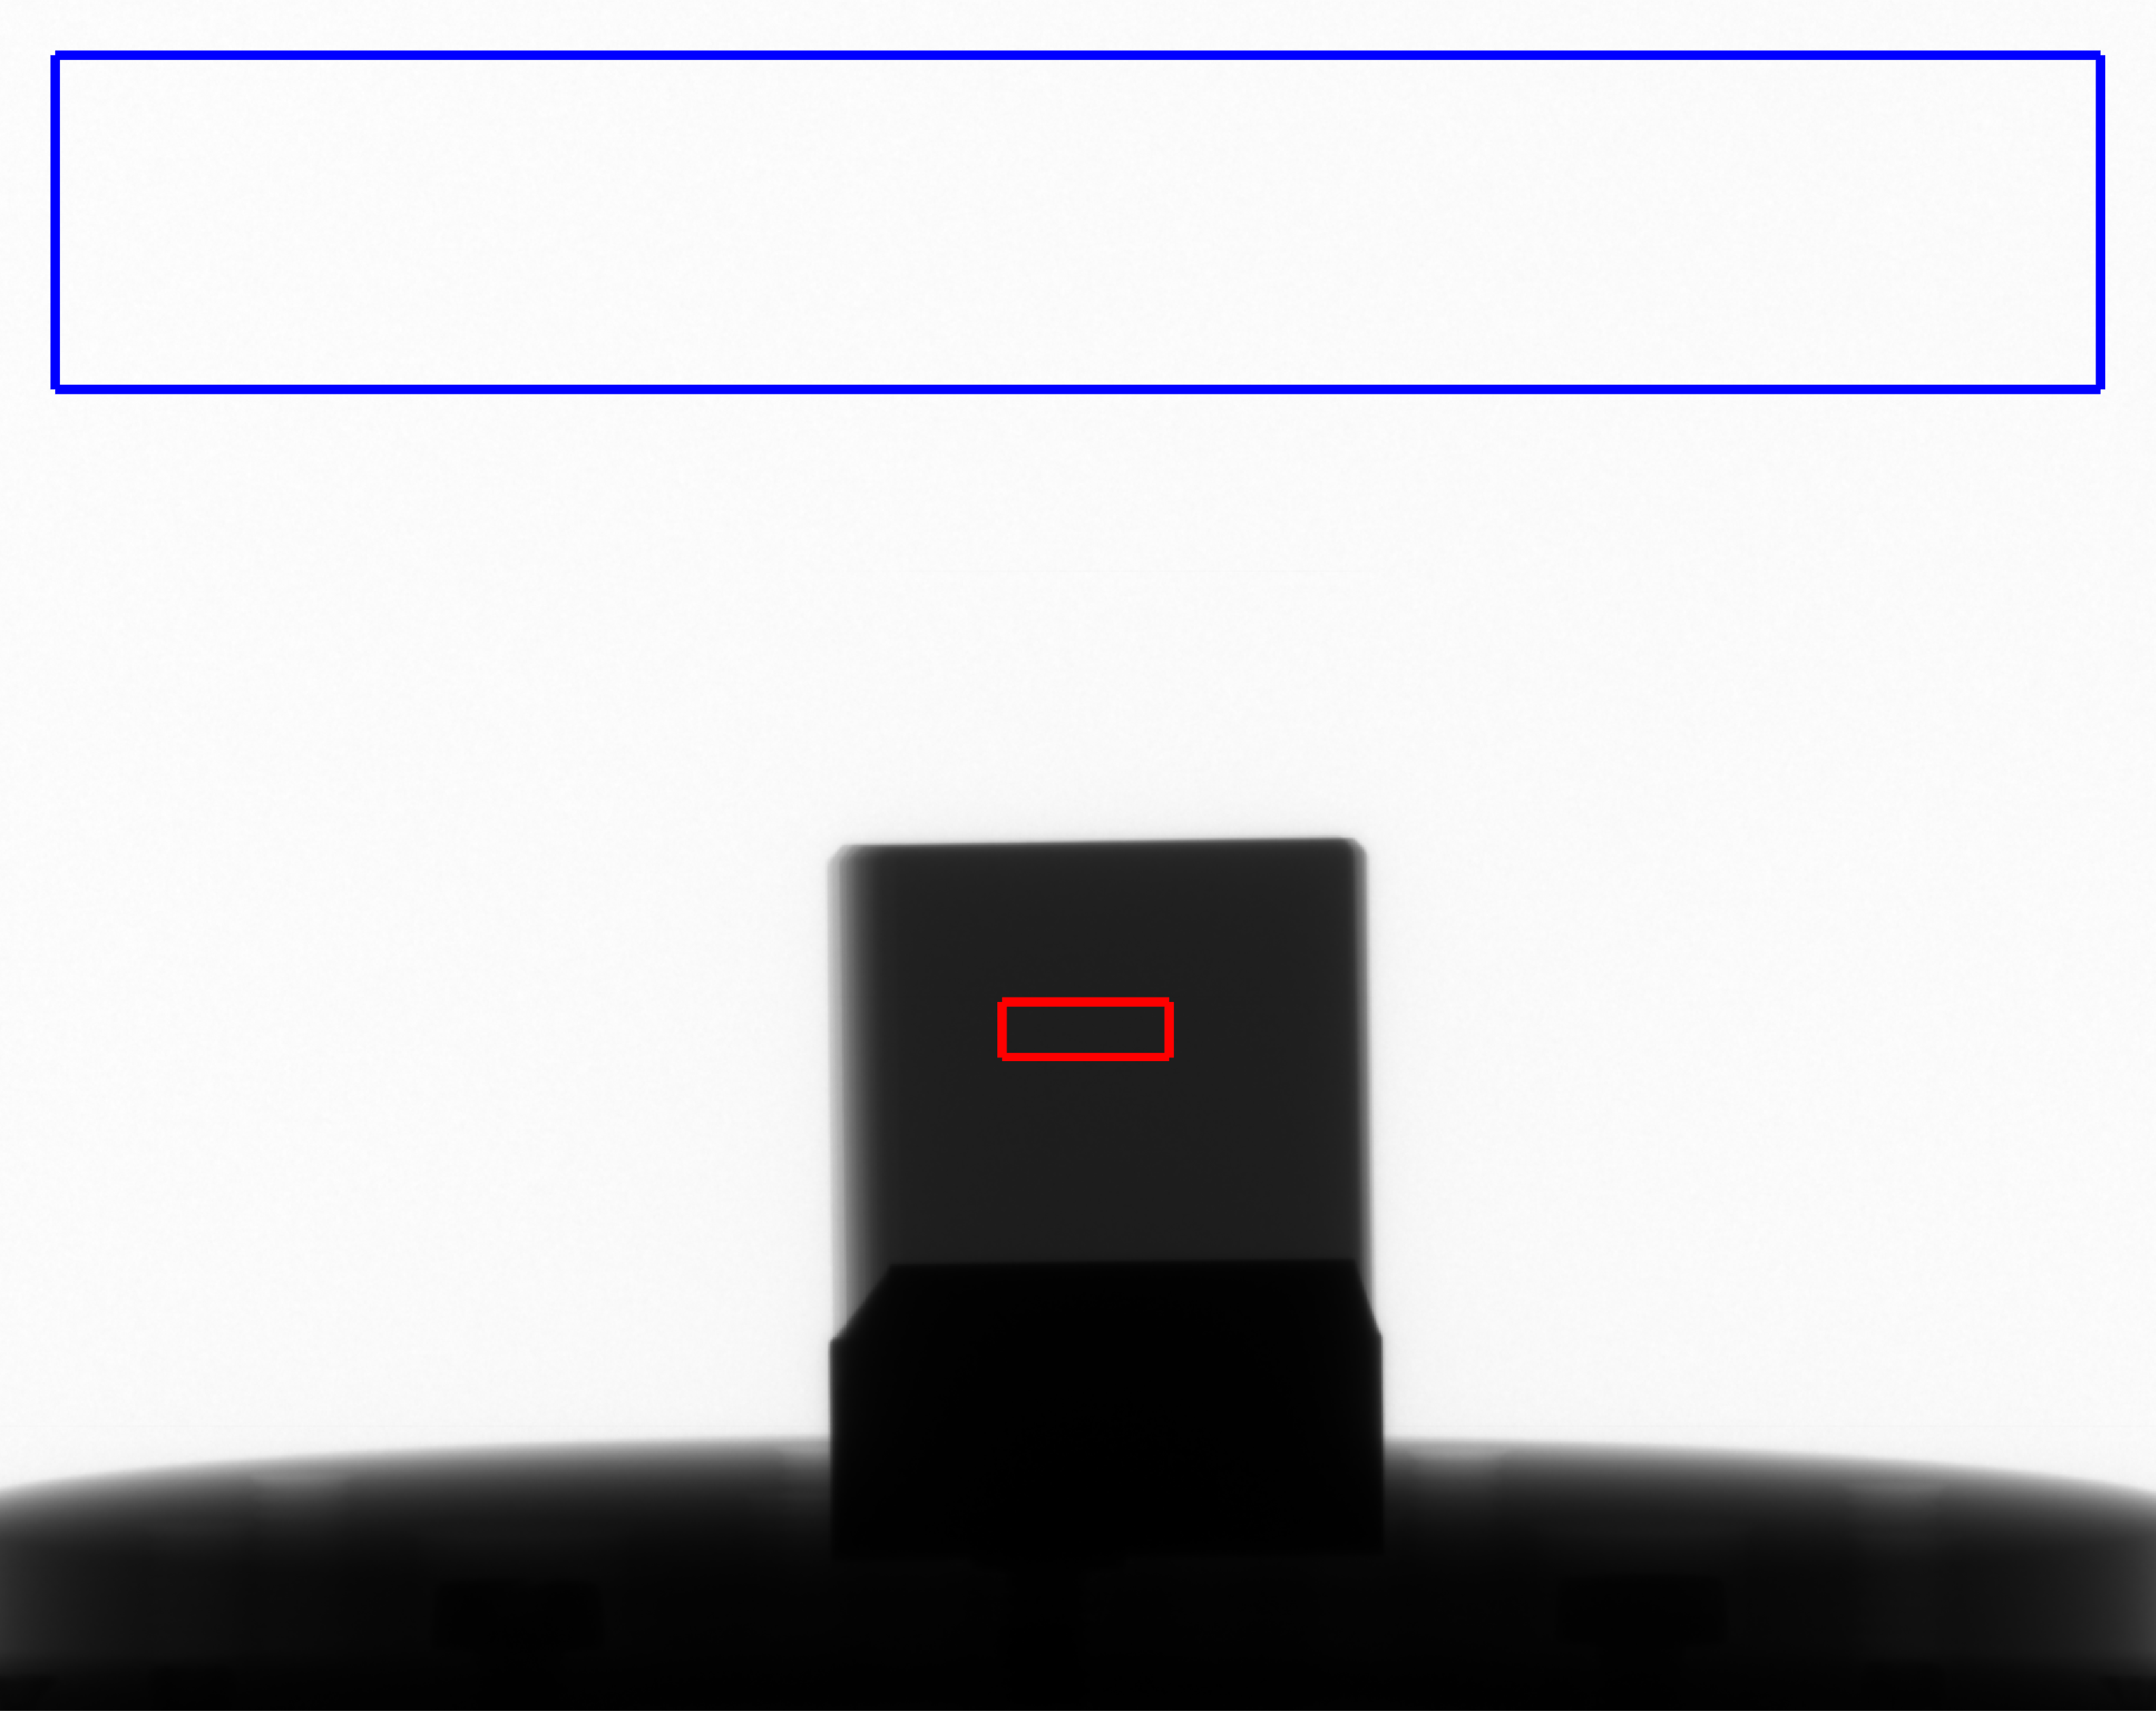
\includegraphics[width=0.8\textwidth]
	{Sources/beam_hardening/20_plates.png}
\end{textblock}



%%% VOLTAGES
\begin{textblock}{0.39}(0.23,0.0)
	\visible<1->{
		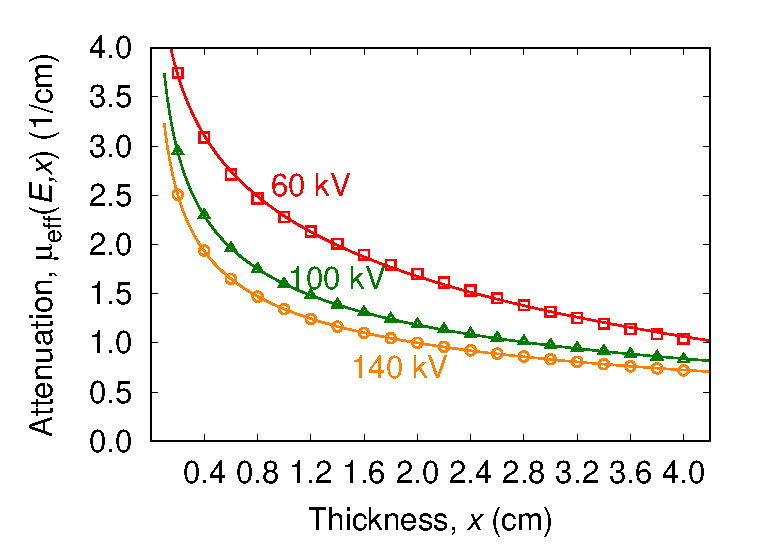
\includegraphics[width=\textwidth]
		{Sources/beam_hardening/borosilicate_glass_voltages_mu_eff.eps}}
\end{textblock}

\begin{textblock}{0.6}(0.23,0.0)
	\vspace{0.5cm}	
	\visible<1->{
		\hspace{3.cm} \colorbox{blue1}{\textcolor{white}{
		 varying voltages}}}
\end{textblock}


%% FILTERS
\begin{textblock}{0.39}(0.62,0.0)
	\visible<2->{
		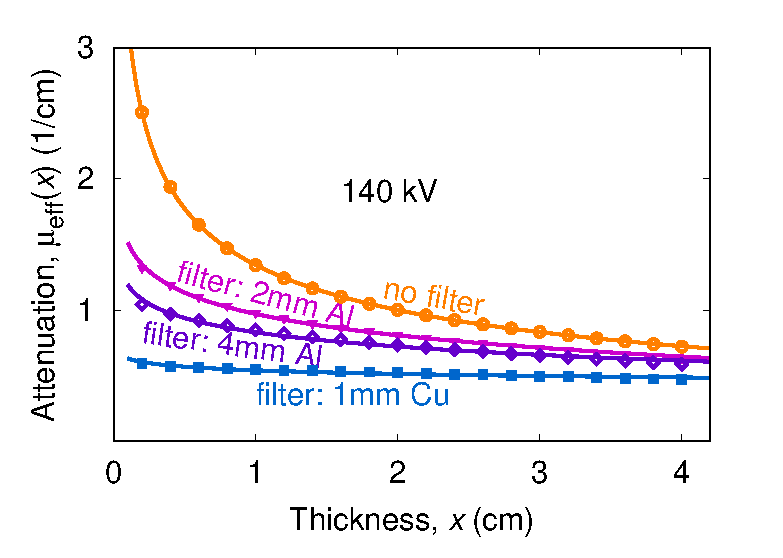
\includegraphics[width=\textwidth]
		{Sources/beam_hardening/borosilicate_glass_filters_mu_eff.eps}}
\end{textblock}

\begin{textblock}{0.6}(0.62,0.0)
	\vspace{0.5cm}	
	\visible<2->{
		\hspace{3.cm} \colorbox{blue1}{\textcolor{white}{
				different filters}}}
\end{textblock}

%% MATERIALS
\begin{textblock}{0.39}(0.23,0.5)
	\visible<3->{
		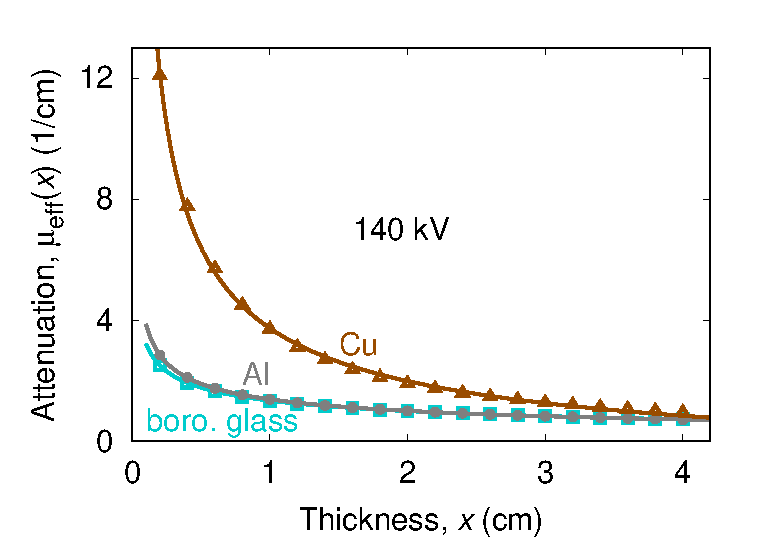
\includegraphics[width=\textwidth]
		{Sources/beam_hardening/materials_mu_eff_140kV_fit.eps}}
\end{textblock}

\begin{textblock}{0.6}(0.23,0.5)
	\vspace{0.5cm}	
	\visible<3->{
		\hspace{3.cm} \colorbox{blue1}{\textcolor{white}{
				different materials}}}
\end{textblock}

%% SETUPS
\begin{textblock}{0.39}(0.62,0.5)
	\visible<4->{
		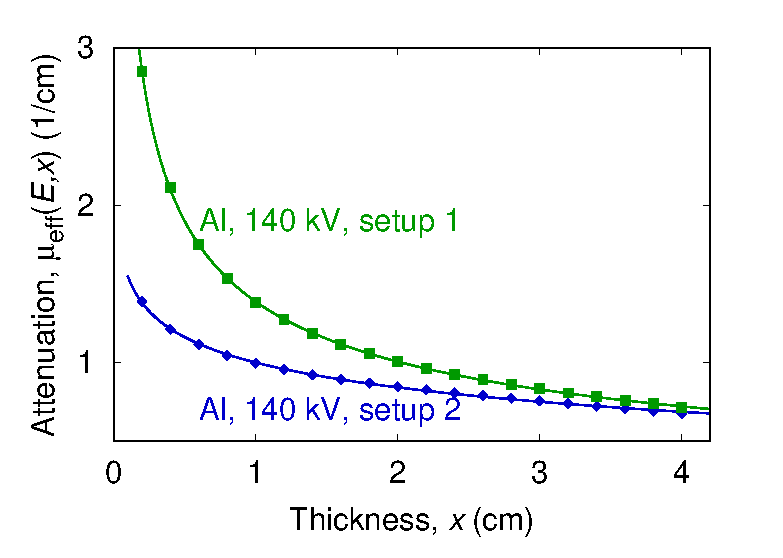
\includegraphics[width=\textwidth]
		{Sources/beam_hardening/comp_both_setups.eps}}
\end{textblock}

\begin{textblock}{0.6}(0.62,0.5)
	\vspace{0.5cm}	
	\visible<4->{
		\hspace{3.cm} \colorbox{blue1}{\textcolor{white}{
				2 X-ray setups}}}
\end{textblock}
}

%% ------------- MATERIAL THICKNESS X
\frame{
\begin{tikzpicture}[remember picture,overlay]
\fill[blue1]
(current page.north west) rectangle ([xshift=0.55\textwidth,yshift=0.34\textheight]current page.west|-{pic cs:end});
\end{tikzpicture}

\begin{textblock}{0.5}(0.02,0.03)
	\textcolor{white}{
		\Large Determining the material thickness $x$}
\end{textblock}


\begin{textblock}{0.5}(0.05,0.15)
\visible<1->{
Generalized Beer-Lambert
\[ I(x) = I_0 \exp(-\mu_\text{eff} (x) \, x) \]

Model function
\[ \mu_\text{eff} (x) = a + \frac{b}{x^\alpha} \]\\[0.5cm]
}

\visible<2->{
Solve
\[ a x + b x^{1-\alpha} + \ln \left(\frac{I(x)}{I_0}\right) = 0\]
e.g.\ Newton's method or look-up table}
\end{textblock}

\begin{textblock}{0.4}(0.55,0.05)
\only<1>{
	\includegraphics[width=\textwidth]
	{Sources/beam_hardening/borosilicate_glass_mueff_3datapoints_multiplot_1.eps}
}

\only<2>{
	\includegraphics[width=\textwidth]
	{Sources/beam_hardening/borosilicate_glass_mueff_3datapoints_multiplot_2.eps}
}

\visible<3->{
	\includegraphics[width=\textwidth]
	{Sources/beam_hardening/borosilicate_glass_mueff_3datapoints_multiplot.eps}
}
\end{textblock}
}

%% ------------- Applications ------------------------
\frame{
\begin{tikzpicture}[remember picture,overlay]
\fill[blue1]
(current page.north west) rectangle ([xshift=1.\paperwidth,yshift=0.33\paperheight]current page.west|-{pic cs:end});
\end{tikzpicture}

\begin{textblock}{1.}(0.02,0.03)
	\textcolor{white}{
		\Large Migrating shear bands in shaken granular matter, Kollmer \textit{et al} (2020)}
\end{textblock}

\begin{textblock}{0.9}(0.05,0.12)
	\centering
	\only<1>{
	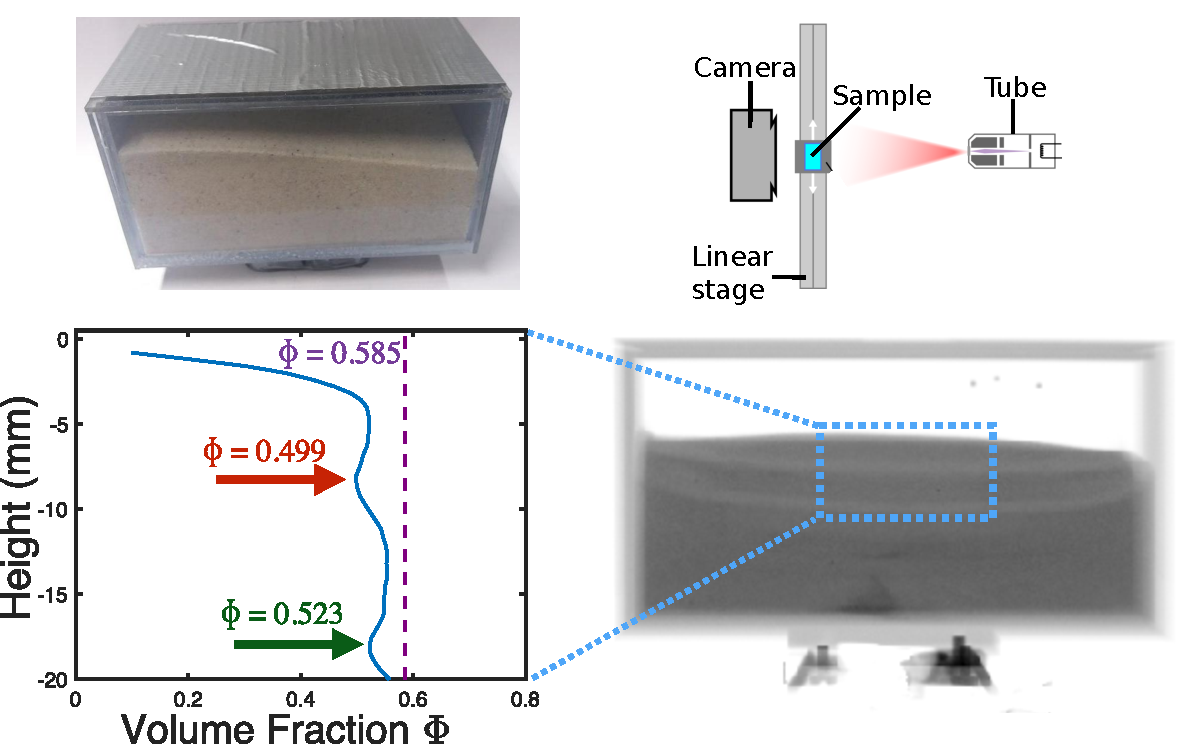
\includegraphics[width=0.8\textwidth]
	{Sources/beam_hardening/migrating_shearband.pdf}}
\end{textblock}
}